\documentclass[a4paper,fleqn]{cas-dc}

% ---- Font and encoding ----
% NOTE: cas-dc.cls loads [notext]{stix} + charis internally (Times-compatible).
% lmodern must NOT be used — it conflicts with cas-dc's font settings.
\usepackage[T1]{fontenc}
\usepackage[utf8]{inputenc}
\usepackage{textcomp}                         % extra T1 text symbols
\pdfgentounicode=1                             % enable ToUnicode CMap
\input{glyphtounicode}                         % standard LaTeX glyph→Unicode map
% ---- Fix critical glyph-to-Unicode mappings in PDF text layer ----
\pdfglyphtounicode{approxequal}{2248}          % ≈
\pdfglyphtounicode{notequal}{2260}             % ≠
\pdfglyphtounicode{proportional}{221D}         % ∝
\pdfglyphtounicode{partialdiff}{2202}          % ∂
\pdfglyphtounicode{gradient}{2207}             % ∇
\pdfglyphtounicode{musicalflat}{266D}          % ♭
\pdfglyphtounicode{sim}{223C}                  % ∼
\pdfglyphtounicode{approx}{2248}               % ≈ (alt name)
\pdfglyphtounicode{leq}{2264}                  % ≤
\pdfglyphtounicode{geq}{2265}                  % ≥
\pdfglyphtounicode{pm}{00B1}                   % ±
\pdfglyphtounicode{times}{00D7}                % ×
\pdfglyphtounicode{cdot}{22C5}                 % ⋅
\pdfglyphtounicode{circ}{2218}                 % ∘
\pdfglyphtounicode{bullet}{2022}               % •
\pdfglyphtounicode{element}{2208}              % ∈
\pdfglyphtounicode{ellipsis}{2026}             % …
\usepackage{amsmath,amssymb,amsfonts}
\usepackage{graphicx}
\usepackage{xcolor}
\usepackage{algorithm}
\usepackage[noend]{algpseudocode}
% Compact algorithm style for double-column
\algrenewcommand\alglinenumber[1]{\footnotesize #1:}
\usepackage{booktabs}
\usepackage{url}
% hyperref is already loaded by cas-dc.cls; loading it a second time is
% unnecessary. Anchor names are made unique instead, so that floats no
% longer emit "destination with the same identifier" warnings.
\hypersetup{hypertexnames=false}
\usepackage{tabularx}
\usepackage[expansion=false]{microtype}
\usepackage{placeins}
\usepackage{float}
\usepackage[authoryear,round,sort]{natbib}


% ---- Spacing ----
\setlength{\abovecaptionskip}{4pt plus 1pt minus 1pt}
\setlength{\belowcaptionskip}{2pt plus 1pt minus 1pt}
\setlength{\floatsep}{8pt plus 3pt minus 3pt}
\setlength{\textfloatsep}{10pt plus 3pt minus 3pt}
\setlength{\intextsep}{8pt plus 3pt minus 3pt}
\renewcommand{\topfraction}{0.88}
\renewcommand{\bottomfraction}{0.75}
\renewcommand{\textfraction}{0.12}
\renewcommand{\floatpagefraction}{0.65}
\setcounter{topnumber}{3}
\setcounter{bottomnumber}{2}
\setcounter{totalnumber}{5}

% ---- TikZ ----
\usepackage{tikz}
\usetikzlibrary{shapes.geometric,arrows.meta,positioning,calc,decorations.pathmorphing,backgrounds,fit,patterns}

\sloppy
\tolerance=2000
\emergencystretch=\columnwidth
\hyphenpenalty=200
\exhyphenpenalty=200

\newcommand{\lambdax}{\lambda_x}
\newcommand{\mflat}{\mathbin{\flat}}
\newcommand{\rhosup}{\sup_{\substack{p\in\mathcal{M},\,v\in T_p\mathcal{M}\\\|v\|=1}}}

\DeclareMathOperator*{\argmin}{argmin}

\begin{document}

% ------------------------------------------------------------
% Paper version: v39 (2026-10-07: F-group curvature sweep redesigned around the correct control variable — window-endpoint conformal deviation; corrected claim SUPPORTED Spearman 0.939 controlled / 1.000 realistic; curvature-monotonic claim kept deleted; deployment c=1.0 blind spot disclosed as limitation)
% Paper version: v40 (2026-10-07: deployed truncated-mode correction now threads the learned curvature c into conformal_factor — the c=1.0 blind spot is removed; the SUPPORTED endpoint-deviation claim is re-run on the unpatched deployed path and extended to all four TU datasets, Spearman 0.998, n=48)
% Paper version: v41 (2026-10-07: wording of the curvature-aware bullet clarified — the in-graph training path already invoked curvature-aware PerStepMetricCorrection, so the dvm.py fix affects only the post-hoc apply_dvm sweep/diagnostic path and changes no reported OM result; no scientific claim altered)
% Paper version: v42 (2026-10-09: P0 — DD table tab:dd_results re-sourced from final_results_DD.json (n=9, post-fix): AMC M=8 (54.5%) now correctly reported 1.9 pt BELOW Full BPTT (56.4%, Wilcoxon p=0.074), replacing the withdrawn "+1.0%" claim; "Not yet re-sourced" flag removed; the DD accuracy claim in the reproducibility checklist rewritten to the verified negative finding. P2 — tab:mc_training_grad epoch-5 row aligned to the labeled verification file mc_gradient_scale_fixcheck.json (ratio 1.3e8, cos -0.367; body text absolute norms and per-step factor updated to match). P1 — tab:truncation_error and tab:mc_ablation confirmed machine-generated by make_v3_tables.py from gradient_error_matrix.json (exact match, no change). No scientific claim about the correction mechanism altered.) NB: the v42 fixcheck alignment was later found to draw on a debug run (n_correction_steps=16 vs 1624 in the canonical file) and is reverted in v43 to the canonical mc_gradient_scale.json.
% Paper version: v43 (2026-10-09: (1) tab:mc_training_grad rebuilt from the canonical, git-committed results_v3/mc_gradient_scale.json (2 seeds, epochs 5/10/15/20): the previous version mixed in two epoch rows with no data source (epochs 1, 2) and magnitude/absolute-norm figures from the debug run mc_gradient_scale_fixcheck.json; the rebuilt table reports ratio and cos for both seeds with no blank cells, and the surrounding narrative is rephrased to match (seed 0 ratio 60-103 and a negative cos at epoch 10; seed 7 mild throughout). (2) Table width fixes: tab:truncation_error and tab:bs_ablation wrapped in \resizebox{\columnwidth}; tab:energy_pareto and tab:nospike_scope promoted to full-width table*. All four overflow warnings from the v42 compile are resolved.)
% Paper version: v44 (2026-10-09: full data audit of all 13 tables + body numbers against source JSONs. Two body-text errors corrected: (a) MUTAG 5-shot paired Wilcoxon p 0.21 -> 0.426 (matches tab:nospike_scope and the independent NoSpikesFixed recompute; 1-shot p=0.0078 and +4.62 pt unchanged); (b) ogbn-arxiv ||x|| 0.15 -> 0.30, which is the value self-consistent with the reported constant lambda in [2.2,2.2] under lambda=2/(1-c||x||^2) at c=1.0 (corroborated by the DD line lambda=2.31<->||x||=0.37). Every other table entry and body figure was re-derived from its source JSON and found exact/consistent — no further claims changed.)
% Paper version: v38 (2026-10-07: four-dataset scope of non-spiking result added; Table~\ref{tab:nospike_scope} confirms No-Spikes>OM is MUTAG-only, n.s. on PROTEINS/NCI1/DD)
% Paper version: v45 (2026-10-10: reformatted for the Neurocomputing target and reframed around the memory-accuracy-energy trade-off. (1) Introduction reframed: Problem Statement now states the three-way trade-off explicitly, "This Work" characterises the trade-off instead of claiming an accuracy win, and Contributions is reorganised so the bounded-error result, the telescoping-identity limit and the measured accuracy/energy costs each get their own item. (2) Highlights rewritten to 5 items, each within Elsevier's 85-character limit (previously 92/100/180/403/273 characters, all over). (3) Abstract compressed from 390 to 218 words, preserving the four findings and all key numbers. (4) Bibliography expanded from 35 to 51 entries with Riemannian/hyperbolic graph learning literature verified against the source PDFs and publisher metadata; all 17 new keys are cited in the body (Amari 1998 was already present but uncited). (5) Three figures added (truncation-window schematic, telescoping identity, energy-accuracy Pareto scatter plotted from tab:energy_pareto) — the paper previously had one figure and thirteen tables. No experimental number was changed.)
% Paper version: v46 (2026-10-10: typesetting cleanup — no experimental number or scientific claim changed. (1) The four remaining Overfull hbox warnings are resolved: the 123.6 pt warning came from the Elsevier template itself (cas-common.sty sets the keyword vtop to 0.25 textwidth and then drops it into a zero-width slot), fixed by appending hss inside that slot so the deliberate overhang is absorbed; the 30.9 pt architecture figure is rescaled from 0.74 to 0.62; the tab:mc_ablation header is shortened to "(transient excluded)"; the tab:sentinel first column is switched from l to p{3.3cm} so "Full BPTT (use_dvm=False)" wraps instead of overflowing. (2) The four "\begin{figure}[htbp]" instances are corrected to "[pos=htbp]": cas-dc redefines figure with a key-value optional argument, so the bare "[htbp]" left the float placement empty and raised "No positions in optional float specifier". (3) The duplicate "\usepackage{hyperref}" is removed (cas-dc already loads it) and hypertexnames=false is set, which clears all 17 "destination with the same identifier" warnings for tables and figures. Compile is now clean: 0 errors, 0 overfull boxes, 0 undefined references, 19 pages.)
% Paper version: v49 (2026-10-10: SCI expert review — three P0 inconsistencies found by machine audit, all corrected against result/stats/significance.json (n=9, paired Wilcoxon, BH-FDR). No accuracy number was changed. (1) Discussion item 'Windowed correction stability' claimed full-chain correction degrades accuracy by 11.3% versus truncated AMC; no comparison in the n=9 data supports 11.3 (the only 11.3-scale entry is AMC M=4 vs GIN, -11.36, an unrelated pair). Replaced with the two measured effects: full-chain correction under full BPTT costs 6.1 pt (79.5->73.4, p=0.039, BH 0.048) and in-window correction costs 6.6 pt (80.6->74.0, p=0.008); the 'windowing stabilises correction' claim is WITHDRAWN because at T=8, M=8 the window spans the whole chain and the two implementations agree to 0.6 pt (p=0.43). (2) The '4.9-point gap' to the ANN baseline contradicted the 11.6 pt stated seven lines earlier in the same section; corrected to 11.6 (AMC M=8 74.0 vs Proto-GNN 85.6, diff=-11.64, p=0.0039). (3) The Limitations bullet 'Lack of significance testing' claimed no significance testing had been done, contradicting the paper's own 25 n=9 / BH-FDR results; rewritten to state what is actually done (paired Wilcoxon + BH-FDR, min attainable p=0.0039) and what the real limitation is (folds are not independent replicates; two load-bearing comparisons are non-significant after correction; no comparison is parameter-matched).
% Paper version: v56 (2026-10-13: experiment-matrix framework redesign + code-defect remediation + No-Spikes rerun.)
%   (1) experiment_matrix_redesign.md: defect register (original D1-D5 + new-implementation N1-N5) and a unified-harness design. Mutual defects verified by git diff + targeted audit.
%   (2) Code fixes (programfiles/): D3/N5 dvm.py — conformal_factor no longer defaults to c=1.0 (now a required arg); apply_dvm threads the real manifold curvature c (defaulting to manifold.c) into the correction and into DvMFunction forward/backward, so the truncated/main-training path is no longer curvature-blind; c=0 -> lambda=2 (exact Euclidean limit). N1 neurons.py — the no_spikes ablation no longer gates the manifold recurrence with a near-zero sigmoid (which froze the state and collapsed the readout): the recurrence now runs unmasked over all T steps and emits a continuous rate proxy that does not gate the state. R1 (regression) — no_spikes spike_mask shape restored to (N,1) (a bare (N,) crashed every ablation via right-aligned broadcast). msg_baseline/manifolds.py — expmap0/logmap0/expmap/logmap/dist return the correct Euclidean limits at c<1e-7 (removes the NaN that previously made c=0 degenerate to a constant readout).
%   (3) verify_suite/verify_ablation_functional.py: CPU functional tests (no GPU/dataset) covering curvature threading, c=0 Euclidean limit, no_spikes state evolution, full-spiking gradient flow; 5/5 pass.
%   (4) Paper L1289 no_spikes mechanism re-described to match the current (unmasked-recurrence) implementation.
%   (5) No-Spikes arm rerun in progress (4 datasets x 9 runs x 100 epochs, task nnuWVd): the N1 fix changed the ablation's behaviour, so the post-fix No-Spikes numbers and the derived gaps/p-values at L1289/1291/1295/1345/1368 are being re-measured and will be updated on completion. OM/full numbers are UNCHANGED by the fixes (c=1.0 gives numerically identical results) and need no rerun.
%   (6) c=0 degenerate (dense Euclidean) baseline investigated as a curvature-control: under the standard few-shot protocol it does NOT train to above-chance accuracy (exactly 0.5 across 3 independent runs) even though its embeddings evolve and its classifier is mathematically correct at c=0; we attribute this to the loss of the curvature-induced optimisation bias. It is dropped; the parameter-matched dense comparison relies on the existing GIN/GCN/SAGE baselines (232,850 params), which are invariant to the fixes.
% Paper version: v57 (2026-10-15..17: No-Spikes rerun under the current unmasked-recurrence code COMPLETED for BOTH 1-shot and 5-shot (4 datasets x 9 runs x 2 shots; 5-shot finished 2026-10-17 via task 1EM61Y, EXIT=0). KEY FINDING: the previously reported MUTAG non-spiking advantage (+7.60 pt, paired Wilcoxon p=0.0078, 8/9 positive) was measured under the EARLIER sigmoid-gated intermediate build and does NOT survive the unmasked-recurrence correction. Under the current code the non-spiking continuous ablation is NOT significantly better than the spiking OnManifold model on ANY dataset, ANY shot: 1-shot gaps MUTAG +3.31 (p=0.652), PROTEINS +0.80 (p=0.156), NCI1 -0.53 (p=0.359), DD +0.22 (p=0.250); 5-shot gaps MUTAG +3.31 (p=0.820), PROTEINS +1.71 (p=0.496), NCI1 +0.11 (p=0.734), DD -0.22 (p=0.570); all non-significant after BH-FDR. The claim is retracted and the section reframed as a clean null result (spike-and-threshold dynamics impose no measured accuracy cost at the studied operating point). Revisions: (a) tab:nospike_scope 1-shot AND 5-shot No-Spk columns + Delta/p updated to fresh values (sample std, ddof=1, matching the OM column convention). (b) body L1296/1298/1302-caption/1352/1375 rewritten to the null-result framing and to withdraw the +7.60/p=0.0078 claim. (c) std convention reconciled: OM columns use sample std (ddof=1); the run-file std_acc is population std (ddof=0) and is converted before table entry. (d) verify_numbers.py now guards tab:nospike_scope via nospike_scope_expected.json (backfill_nospike.py emits it, flags stale/pre-fix files by neurons.py mtime); all 8 cells green post-1EM61Y.
% Paper version: v58 (2026-10-17: post-review revision). (1) P0: removed the Experimental Setup claim that significance testing was "deferred to an extended technical report" (it contradicted the paper's own paired Wilcoxon + BH-FDR analysis); now states every comparison IS tested and n=9 = 3 seeds x 3 folds. (2) P1: fixed the four-TUDatasets enumeration (was MUTAG/DD/PROTEINS/ENZYMES) to MUTAG/PROTEINS/NCI1/DD in Contributions(vi), validation-pipeline sentence, and Data Availability; ENZYMES retained only as the excluded negative-result dataset. (3) P1: completed the Data-Availability JSON list and made L1169 name all carrying datasets.
% Paper version: v59 (2026-10-17: multi-skill joint review). Ran all six local review
%   skills (academic-review-revisor, academic-integrity-checker, paper-code-data-consistency-audit,
%   academic-citation, final-integrity-check, latex-manuscript-hygiene). Fixes: (1) Highlights
%   item 1 trimmed to <=85 chars (Elsevier limit; was 129) while keeping O(M) stored states +
%   measured peak bytes. (2) tab:positive_interval now cited in body (subsec 'The positive
%   interval'); its 'AMC gain' column header clarified to 'AMC gain (uncorr.-AMC)'. All other
%   review findings were PASS (0 dangling citations, clean tex structure, machine-consistency
%   suite green, all mandatory declarations present). No accuracy number changed.
% Paper version: v60 (2026-10-18: math-logic audit revisions per post/math_audit_report.md. P0 -- reframed Eq.main_correction and Theorem 2 as the AMC correction OPERATOR rather than the textbook Riemannian pullback; added Remark (round-trip cancellation) proving the canonical Riemannian/autograd gradient carries no conformal factor, so the per-step multiplier is a defined re-scaling, not the canonical pullback; weakened the 'AMC reproduces the true Riemannian gradient' claim (M=T sentinel is internal-consistency, circular). P1 -- qualified the positive-interval 'cosine 1.0 in every cell' claim to the radial synthetic chain only. P2 -- clarified the uniform C bound's domain of validity (lambda_x <= 2/(c epsilon) requires c <= 4/(1+epsilon)^2, satisfied by c=1 used in all experiments). Softened 'Riemannian metric correction' framing in abstract/intro/contributions/algorithm to 'conformal correction operator'. No accuracy number or table changed; the v59 snapshot remains the canonical v59 source.
% v37 (2026-10-03: w/o Spikes post-fix disclosure — line 862 rewritten;
%               new paragraph in Sec."Accuracy Relative to Non-Spiking Baselines";
%               Conclusion negative result (iv) added; non-spiking continuous
%               ablation now REPORTED (not excluded) at 79.27/84.71; its nominal
%               100% energy figure flagged as a zero-numerator accounting artefact)
% v36 (Phase-4: narrative reframed around an energy--accuracy
%               trade-off; Conclusion contradiction with the body fixed
%               (old text claimed full-BPTT parity and a +3.2pt DD metric-
%               correction advantage, both withdrawn in the body); new
%               Sec."Energy--Accuracy Pareto" with analytical energy model;
%               "w/o Spikes" 50% collapse traced to missing no_spikes branch
%               (NaN), FIXED post-fix to 79.27/84.71 and now REPORTED (not
%               excluded): non-spiking continuous ablation beats spiking
%               OnManifold on MUTAG 1-shot by +7.60pt, paired Wilcoxon p=0.0078;
%               its nominal 100% energy "saving" is a zero-numerator artefact)
% v35 (Phase-3: all accuracy numbers re-sourced to the
%               post-fix n=9 reruns; metric-correction harm reported)
%   - Renamed: Differentiation-via-Manifold (DvM) -> Analytic Metric Correction (AMC)
%   - Added Sec.1 "Provenance and Relationship to MSG" disclosure
%   - Fixed 6 erroneous bibliography entries (verified against paper/ PDFs)
%   - Verified externally (arXiv/OpenAlex/Crossref): Roy19 real (paywalled, metadata
%     exact); Ganev19 hallucinated -> bibitem deleted, citation folded into Becigneul19
%   - Replaced untraceable batch-size numbers with batch_ablation_30ep.json
%   - Theorem numbering: Thm.1 = error bound (Sec.4.1), Thm.2 = chain rule (App.)
%   - Hardcoded table numbers replaced by \ref; empty Sec.4.2 filled in
% v33 (Phase 0, no new experiments required):
%   - P0-D: Eq.(1) now carries the lambda_0^2/lambda_T^2 factor consistently with
%     Eq.(11) and Corollary 1; C redefined accordingly; "independent of T" weakened
%     to "uniformly bounded in T under the stability projection".
%   - P1-1: Algorithm 2 (truncated variant) is now referenced in the main text.
%   - P1-3: ENZYMES random-baseline disclosure (20% vs 23.5%; AMC == full BPTT).
%   - P1-2: PROTEINS 57.3% source and accounting explicitly stated.
%   - P1-4: Discussion now answers Proto-GNN(ANN) 85.6% > AMC 74.0%.
%   - P2-3: cosine > 1 floating-point display corrected.
%   - New limitation: AMC does not backpropagate to the MSPE input projection
%     when M < T (measured; see Sec. Limitations).
% ------------------------------------------------------------
%   v47 (2026-10-10) — Table 12 provenance, stated as it actually happened.
%     No experimental number was changed. What changed is the disclosure:
%     (a) The 71.7% in Table 12 was measured on the 28-config matrix OM arm
%         (100 epochs, T=M=8, metric correction ON); the 79.5% "Full BPTT" in
%         Table 4 is a different arm (50 epochs, DvM operator bypassed, no
%         correction). Both are real; the 7.8-point gap is decomposed into the
%         measured correction cost (6.6 pt) plus the 50->100 epoch difference
%         (1.7 pt), so the two figures are not in conflict.
%     (b) Disclosed that at T=M=8 the truncation window spans the whole
%         sequence, so no truncation occurs on that arm; the accuracy cost of
%         genuine truncation is the separate M=8 -> M=4 drop (2.7 pt).
%     (c) Table 12 caption no longer says "full" in a way that reads as full
%         BPTT; the Euclidean comparison column is GIN throughout (the previous
%         "Best Eucl. GNN" header disagreed with its own caption on DD).
%     (d) Table 4 attribution note separates correction cost from truncation
%         cost. Reported results and significance claims are unchanged.
%   v48 (2026-10-10) — the "AMC truncated M=8" label is now actually fixed.
%     v47 only added an explanatory paragraph; the table rows still read
%     "AMC truncated M=8". Because T=8 on the TU benchmarks, M=8 gives
%     start_idx = max(0, T-M) = 0, so no state is discarded and the label was
%     false. Changes (no experimental number altered anywhere):
%     (a) Tables 4 (MUTAG) and 5 (DD): the two M=8 rows become
%         "AMC M=8 <dag>" / "No Correction M=8 <dag>", dagger explained in each
%         caption; the M=4 row keeps "truncated" (only genuinely truncated one).
%     (b) One global convention declared where the window is introduced, so every
%         later "AMC M=8" figure is read correctly.
%     (c) tab:msg_comparison row marked with the same dagger + inline note.
%     (d) fig:architecture caption now says the saving requires T > M.
%     (e) Conclusion: "storing M+1=9 states instead of T" was false at T=8
%         (9 >= 8, nothing saved); now attributes the 5.5-pt gap to the
%         correction and states the saving realises only for T >> M (14x @128).
%     (f) Both verified-claim entries carry the same qualifier.
%     NOTE: M=8 IS genuinely truncated wherever T > 8 (T=16 diagnostics,
%     T=128 scaling); those are untouched.
%   v50 (2026-10-10) — structural defect found during the post-desk-reject
%     compliance sweep: the Reproducibility Checklist (an appendix-level
%     \section) was typeset INSIDE the thebibliography environment, because
%     \end{thebibliography} sat after it rather than before it. Every checklist
%     item was therefore being rendered as part of the reference list, and the
%     \citep calls inside it resolved from inside a bibliography context.
%     Fixed by closing the bibliography before the checklist section.
%     No experimental number, table, or scientific claim was changed.
%     Verified: pdflatex x3, 0 errors / 0 Overfull / 0 undefined refs /
%     0 duplicate destinations.
%   v53 (2026-10-12) — narrow the "O(M) memory" wording to "O(M) stored states"
%     across the front matter (abstract L236, This Work L271, Contributions L278,
%     Conclusion L1170/L1176, highlights L227) following the measured finding that
%     peak GPU bytes are O(T) in this implementation (Table~\\ref{tab:measured_om}),
%     so the O(M) bound governs stored states, not measured bytes. This aligns the
%     wording with the Limitations bullet added in v52. No number or other claim
%     was changed.
%   v55 (2026-10-13) — P0-B: byte-level O(M) now MEASURED (true peak-GPU-byte O(M)),
%     not merely a stored-state bound. Engineering: STMP window-exterior steps
%     (t < start_idx = max(0, T - M)) now run under torch.no_grad, so the retained
%     autograd graph spans only the last M steps and peak bytes scale with M, not T.
%     (Detaching only the state tensor p_hyp did NOT reduce peak -- autograd still
%     saved RGC/LIF intermediate activations; the no_grad wrapper is what works.)
%     T == M is a structural no-op, so the reported T = M = 8 path is byte-identical
%     (verify_p0b.py Part 0: max|grad| diff = 0.000, and _window_detach == False
%     because start_idx == 0). Evidence: verify_p0b.py paper-scale T=32 900.6 -> 316.6 MB
%     and T=64 1784.5 -> 541.9 MB (2.8-3.3x); real MUTAG T-sweep (run_T_sweep.py with
%     truncate_memory=True) T=32 truncated 105.6 MB vs full-BPTT 271.9 MB; T=64
%     truncated 160.1 MB vs full-BPTT 522.7 MB (2.6-3.3x). P0-B is gated
%     behind config.truncate_memory (default True). verify_p0b.py added to check_all.sh
%     as the 5th machine check. Edits: highlight L283, Contributions L334, figure node
%     L571, Stage 4 memory L796, tab:measured_om caption L818 and cells L826-829,
%     Limitations L1302, Conclusion L1307/L1313 -- all flipped from "byte-level O(M)
%     is future work / peak is O(T)" to "byte-level O(M) now measured". No accuracy
%     number was changed at T = M = 8 (Part 0 proves the path identical); only the
%     long-T peak table is refreshed with the new measurements.
%   v54 (2026-10-12) — SCI review (papersh) action items C, D and the four-fold
%     machine-verification suite. No accuracy number was changed.
%     (C) New Table tab:positive_interval + "The positive interval: where the
%         correction is indispensable" narrative (sec:when_mc_matters): a synthetic
%         hyperbolic-hierarchy chain on the Poincare ball with a controlled endpoint
%         conformal ratio lambda_T/lambda_0 in {1.01,1.06,1.27,2.05,4.63}. The
%         AMC-corrected truncated gradient keeps a dispersion-INDEPENDENT error
%         ceiling of 1-rho^(T-M)=0.57 (cosine 1.0 to full-BPTT ground truth), while
%         the uncorrected truncated gradient has no ceiling and diverges to rel_err
%         8.21 (an 8x mismatch) at lambda_T/lambda_0=4.63. This closes the R2 gap:
%         the correction is a no-op at the near-identity TU working point but is the
%         only safe choice where embeddings are dispersed. Source run_positive_interval.py
%         -> positive_interval.json (T=16, M=8, c=1, 20 trials).
%     (D) Parameter-matched 5-variant SpikeRPGNN matrix confirmed: every row of
%         tab:gnn_results / tab:dd_results is the same architecture under a different
%         training-time gradient treatment (identical config in run_final_matrix.py:
%         hidden=128, layers=3, tau=20, lr=1e-3, wd=5e-4, c=1.0; only dvm_mode /
%         dv_m_window / use_metric_correction differ). Numbers verified == JSON.
%     (Suite) Four-fold machine-verification suite shipped under verify_suite/ and
%         runnable via `bash verify_suite/check_all.sh` (passes). It caught a REAL
%         hyperparameter drift: the manuscript setup said "no weight decay" but the
%         executed config used weight_decay=5e-4; the setup is now corrected to
%         "weight decay 5e-4" (L1620). Audit: audit_data (n=9, no NaN), verify_numbers
%         (30 table values traced to JSON), verify_hyperparams (runtime reflection),
%         verify_algorithm_mapping (pseudocode<->implementation fingerprinting with
%         negative controls). Reproducibility Notes now cites the suite.
%   v52 (2026-10-12) — supplementary T=32/64 measurement experiment answering
%     R2's "T=8=M=8 makes truncation vacuous" objection with REAL bytes, not the
%     synthetic state-count of v51. Four-cell MUTAG sweep (T in {32,64} x
%     {truncated M=8, full BPTT M=T}, single seed, 3 epochs; peak =
%     torch.cuda.max_memory_allocated). FINDING (honest, two-sided):
%     (a) MEMORY: measured peak bytes are nearly identical between the two
%         regimes (287 vs 272 MB at T=32; 556 vs 523 MB at T=64) because the
%         forward pass stacks all T hidden states for temporal pooling, so live
%         allocation is O(T) regardless of M. The O(M) bound therefore governs
%         STORED BACKWARD-HISTORY STATES (the 14x figure in tab:scaling), not
%         measured peak bytes in this implementation. This corrects the earlier
%         implication that O(M) reduces peak GPU memory; byte-level savings would
%         need gradient checkpointing / forward chunking (future work).
%     (b) STABILITY: truncated trains stably to T=64 (69.4% after 3 ep) while
%         full BPTT aborts with a NaN there — evidence that the windowed metric
%         correction + contraction decay keep long-horizon training stable.
%     Edits: new Table tab:measured_om (real peak MB + outcome); Stage 4 memory
%     paragraph now states O(M) is a stored-state bound and reports the measured
%     O(T) bytes; new Limitations bullet makes "O(M) memory" explicit as a
%     stored-state bound, not a measured byte reduction. No accuracy number was
%     changed. Verified: gen_measured_table.py reads T_sweep_MUTAG.json; values
%     cross-checked against the sweep log. (Full T=32/64 accuracy sweep ~hundreds
%     of GPU-hours was judged infeasible on this machine and is NOT claimed.)
%   v51 (2026-10-10) — point-by-point response to the Neurocomputing reviewer
%     reports (R2 dated Sep 7, R1 dated Sep 16). No experimental number was
%     changed; no accuracy figure was touched. Seven edits:
%     (1) SLTT bibitem title was wrong — replaced with the real published
%         title "Towards memory- and time-efficient backpropagation for
%         training spiking neural networks", ICCV 2023 (verified against
%         arXiv:2302.14311, whose author list matches our entry exactly).
%     (2) R2-1: SLTT now expanded at first occurrence as "Spatial Learning
%         Through Time (SLTT)" (full name verified in the source abstract).
%     (3) R2-7: the manifold-scope paragraph now states explicitly that the
%         learnable parameters are Euclidean and NOT on the manifold; only
%         the recurrent state is.
%     (4) R2-5: the Conclusion now separates the scope of the mechanism
%         (general recurrent transitions, no spiking-specific property used)
%         from the scope of the empirical claims (the single spiking
%         architecture; no transfer asserted to other recurrent models).
%     (5)(6) Residual "DvM" labels in the body renamed to AMC, so body text
%         and table row labels agree (R1 objected to the DvM name).
%     (7) R2-3: Table 4 caption now states that every row except the last is
%         the same SpikeRPGNN architecture under a different training-time
%         gradient treatment; Proto-GNN (ANN) is the non-spiking reference.
%     R1 items already fixed in v35-v49 and re-verified here: MSG bibitem is
%     now Sun, L., Huang, Z., Wan, Q., Peng, H., & Yu, P. S. (NeurIPS 2024);
%     the Provenance and Relationship to MSG paragraph attributes the term
%     and the problem framing; the two duplicate "Theorem 1" are now
%     Theorem 1 (error bound, proved in Sec. 4.1) and Theorem 2 (chain rule,
%     proved in the appendix); Sec. 4.1 now carries an explicit theorem
%     statement before the proof. R2-2 (empty 4.2), R2-4 (how M is chosen),
%     R2-6 (Theorem ??) were already fixed and re-verified.
%     Verified: pdflatex x3, 0 errors / 0 Overfull / 0 undefined refs /
%     0 duplicate destinations.
\newcommand{\paperVersion}{v53}

\shorttitle{AMC: Analytic Metric Correction for Truncated BPTT}
\shortauthors{Anonymous}

\title[mode=title]{Analytic Metric Correction: Memory-Efficient Gradient Computation on Riemannian Manifolds for Spiking Networks}

\author[1]{Anonymous}%
\cormark[1]
\ead{Anonymous@qq.com}
\orcidauthor{Anonymous ID} {1}


\affiliation[1]{organization={Anonymous University},
                addressline={Anonymous District},
                city={Anonymous City},
                postcode={Anonymous Num},
                country={Anonymous Country}}

\cortext[cor1]{Corresponding author}

% ------------------------------------------------------------
\begin{highlights}
\item Truncated BPTT plus analytic Riemannian correction: O(M) stored states, peak bytes
\item Gradient error bounded by C(1-rho$^{T-M}$), uniformly bounded in the length T
\item Per-step correction telescopes to an endpoint ratio of conformal factors
\item 14x fewer stored states and 89-99.2\% less estimated energy at 5.5 pt cost
\item Negative results kept in full: STMP silent on 3 of 4 datasets, no accuracy win
\end{highlights}

% ------------------------------------------------------------
\begin{abstract}
Training spiking neural networks on Riemannian manifolds requires backpropagation through time (BPTT), whose memory grows linearly with the sequence length. We treat this as a three-way memory--accuracy--energy trade-off and report all three sides. Analytic Metric Correction (AMC) replaces full BPTT with truncated backpropagation plus an analytic conformal correction operator (the AMC correction), giving $O(M)$ stored states: fourteen times fewer states at $T{=}128$. We prove the gradient error is bounded by $C(1-\rho^{T-M})$ with $C$ uniformly bounded in $T$, and confirm the bound's shape on the real model (maximum relative error $6.3\times10^{-4}$ over 56 units; exact agreement with the full-window AMC reference at $M{=}T$) without claiming tightness, and without claiming the correction equals the textbook Riemannian pullback (Remark in \S\ref{sec:method}). The accuracy side is measured rather than assumed: AMC is 5.5 points below full BPTT on MUTAG ($p{=}0.048$) and 6.6 points below the no-correction control, reaching $74.0\%$ against $53.8\%$ for the MSG baseline and $85.6\%$ for a dense ANN encoder. Under an analytical energy model the spiking model uses $89$--$99.2\%$ less \emph{estimated} energy, yet the STMP stage is silent on three of four datasets, where accuracy collapses to chance. A mechanism result bounds what the correction can deliver: it telescopes exactly to the endpoint ratio $\lambda_0^2/\lambda_T^2$ and is near-identity once trajectories reach a stationary norm (median $|\Delta\cos|=3\times10^{-6}$ over 260 measurements). We withdraw an earlier claim of 46-percentage-point degradation from removing the correction.
\end{abstract}

\begin{keywords}
Riemannian manifolds \sep truncated BPTT \sep memory-efficient training \sep metric correction \sep hyperbolic geometry \sep graph neural networks
\end{keywords}

\maketitle

% ------------------------------------------------------------
\section{Introduction}
\label{sec:intro}

\subsection{Problem Statement}

Backpropagation through time (BPTT) is the standard algorithm for training recurrent neural architectures, including spiking neural networks (SNNs). For a sequence of length $T$, BPTT stores activations at every time step, yielding $O(T)$ memory complexity. This is a well-known bottleneck that limits sequence length and model depth, particularly on resource-constrained hardware.

When the recurrent computation operates on a \textit{Riemannian manifold}, the memory problem is compounded: each time step involves expensive exponential map $\exp_p: T_p\mathcal{M} \to \mathcal{M}$ and logarithmic map $\log_p: \mathcal{M} \to T_p\mathcal{M}$ operations. These geometric primitives cannot be efficiently recomputed during backward pass (as done in gradient checkpointing~\citep{Chen16Checkpoint}) because they involve nonlinear operations (hyperbolic trigonometric functions, M\"obius addition) with non-trivial numerical stability constraints.

\textbf{The question we ask.} Memory, accuracy, and energy are not independently optimizable in this setting, and the three pull against each other. Truncating the recurrence saves memory but biases the gradient. The AMC conformal correction that re-anchors the metric factor costs an additional operation at every step. And the spiking pathway that supplies the energy saving is the same pathway whose silence collapses accuracy on three of the four datasets we study. This paper therefore does \emph{not} present a method that wins on accuracy. We treat the design as a \emph{three-way memory--accuracy--energy trade-off} and report all three sides: we prove that the memory saving comes with a gradient error that is \emph{bounded}---and, under a stability projection, uniformly bounded in the sequence length $T$; we measure what the accuracy side actually costs; and we show that the metric correction, the component one would expect to supply the accuracy, telescopes exactly to an endpoint ratio and is therefore near-identity at our operating points. Characterising where this trade-off is favourable, and where it is not, is the contribution.

\subsection{Related Work and Gap}

\textbf{Memory-Efficient SNN Training.} Direct training of SNNs relies on surrogate-gradient backpropagation, pioneered by STBP~\citep{Wu18STBP} and formalized in the surrogate-gradient learning framework~\citep{Neftci19}, with scalable implementations such as SuperSpike~\citep{Zenke18} and SLAYER~\citep{Shrestha18}. Spatial Learning Through Time (SLTT)~\citep{Meng23SLTT} achieves $O(1)$ memory for SNNs by decoupling temporal gradient propagation into layer-wise local learning signals. However, SLTT is restricted to Euclidean space and provides no mechanism for maintaining gradient consistency across manifold tangent spaces. Concurrent SNN training advances~\citep{Fang21,Deng21,Eshraghian23,Zheng21,Roy19} have similarly focused on Euclidean architectures and do not address the metric distortion challenge.

\textbf{Truncated BPTT.} Classical truncated BPTT~\citep{Williams90} limits backpropagation to the last $M$ steps, achieving $O(M)$ memory at the cost of biased gradients. Various corrections have been proposed for Euclidean RNNs~\citep{Tallec17,Kag19}, but none address the metric distortion introduced by curved manifolds.

\textbf{Riemannian Optimization.} Bonnabel~\citep{Bonnabel13} established Riemannian stochastic gradient descent (RSGD) convergence theory, extended by adaptive variants RAdam~\citep{Becigneul19} and the Geoopt library~\citep{Kochurov20}. The wider programme of moving optimisation from Euclidean space onto manifolds, of which the classical natural-gradient perspective~\citep{Amari98} is an early instance, is surveyed in~\citep{Fei23}. However, RSGD and its variants are optimization algorithms for static parameters---they correct the optimizer step direction, not the temporal gradient propagation through dynamic state sequences---and do not address the chain rule on manifolds.

\textbf{Hyperbolic Deep Learning.} Geometric deep learning~\citep{Bronstein17,Bronstein21} situates graph representation learning within a unified framework for non-Euclidean domains;~\citet{Han25Survey} survey the resulting family of geometric graph neural networks. Message-passing neural networks~\citep{Gilmer17}, instantiated as GCN~\citep{Kipf17}, GraphSAGE~\citep{Hamilton17}, GAT~\citep{Velickovic18}, GIN~\citep{Xu19} and the simplified linear variant SGC~\citep{Wu19SGC}, underpin modern graph learning; whether such classic architectures remain competitive baselines for graph-level tasks is examined in~\citep{Luo25}. Foundational work by Nickel and Kiela~\citep{Nickel17,Nickel18Lorentz} introduced hyperbolic embeddings for hierarchical representations, in the Poincar\'e ball and in the Lorentz model respectively. Subsequent work adapted neural network layers to hyperbolic space~\citep{Ganea18,Mathieu19} and extended graph neural networks to constant-curvature manifolds~\citep{Chami19,Liu19,Bachmann20}, made the curvature adaptive~\citep{Fu21ACEHGNN,Fu23Hyperbolic}, and fused several manifold components within one architecture~\citep{Deng23FMGNN}. Because product manifolds mix curvature components inside a single representation~\citep{Gu19Product,Skopek20,McNeela25}, they are the natural setting for our $H^{d_h} \times \mathbb{R}^{d_e}$ states, and recent Riemannian graph models~\citep{Sun24RMGN,Sun25RiemannGFM} build on exactly this structure; manifold-valued graph inputs are treated in~\citep{Hanik25ManifoldGCN}. Manifold ODEs~\citep{Lou20} explore continuous-time dynamics. These methods operate in hyperbolic geometry for representation learning but do not address temporal gradient propagation, which is the focus of this paper.

\textbf{Manifold Spiking Networks.} The most closely related architecture is MSG~\citep{Sun24MSG} (NeurIPS 2024), which introduced manifold-valued spiking neurons for graph learning. MSG uses standard BPTT with $O(T)$ memory and does not address the gradient truncation problem. In the Euclidean domain, spiking graph networks such as SpikingGCN~\citep{Zhu22} have demonstrated the viability of graph-structured temporal processing. Prior work has also combined hyperbolic representation learning with spiking neural networks; such approaches target hyperbolic encoding for static SNN inputs rather than gradient computation through recurrent manifold state transitions. AMC is complementary to these works: it can be integrated into any manifold-valued recurrent architecture (including MSG's MSNeuron and the hyperbolic SNN models above) to provide memory-efficient training without modifying the forward dynamics.

\textbf{Provenance and Relationship to MSG.} We record the origin of this work explicitly. Our initial motivation---namely, differentiating through manifold-valued recurrent state---and the framing of the problem are inspired by MSG~\citep{Sun24MSG}, which introduced manifold-valued spiking neurons and trained them with standard BPTT. We therefore attribute to MSG the formulation of manifold-valued spiking neurons that this work builds upon. This paper does \emph{not} claim credit for introducing manifold-valued spiking neurons, nor for the phrase ``differentiation via manifold''; we adopt the neutral name AMC throughout precisely to avoid confusion with the terminology introduced in~\citep{Sun24MSG}. The specific contribution we add is, to the best of our knowledge, (i) the replacement of MSG's full BPTT by truncated BPTT, (ii) an analytically derived conformal correction operator whose metric action telescopes exactly (the AMC correction), and (iii) a bound on the resulting gradient approximation error, where the correction is treated as a defined operator rather than as the canonical Riemannian pullback.

\textbf{This Work.} We characterise the memory--accuracy--energy trade-off of training manifold-valued spiking networks under truncated BPTT, rather than claiming an accuracy win for a new method. Concretely, AMC replaces full BPTT by truncated BPTT and applies an analytic conformal correction operator, giving $O(M)$ stored states independent of $T$; we prove that the induced gradient error is bounded by $C(1-\rho^{T-M})$ with $C$ uniformly bounded in $T$; and we establish a mechanism result that bounds what \emph{any} such correction can deliver, namely that the per-step correction telescopes exactly to the endpoint ratio $\lambda_0^2/\lambda_T^2$ and is consequently near-identity whenever the trajectory has reached a stationary norm. We then report the accuracy and energy consequences of this trade-off in full, including the regimes in which it is unfavourable.

\subsection{Contributions}

\begin{enumerate}
    \item \textbf{Analytical Metric Correction.} We define an analytic conformal correction \emph{operator} and derive its exact telescoping property: the per-step multiplier $\lambda_t^2/\lambda_{t+1}^2$ collapses to the endpoint ratio $\lambda_0^2/\lambda_T^2$, independent of the curvature and the intermediate states. We analyse this operator directly and measure its effect empirically, rather than asserting equality with the textbook Riemannian pullback (Remark~\ref{rem:roundtrip}).
    
    \item \textbf{AMC Gradient Mechanism.} We present the complete pushforward/pullback algorithm (Algorithm~1) with per-step metric correction, and its $O(M)$ truncated variant: window-exterior steps are detached from the autograd graph (spikergnn/stmp.py), so the retained graph spans only the last $M$ steps and the peak GPU allocation is $O(M)$ bytes, not $O(T)$.
    
    \item \textbf{Error Analysis: the memory side of the trade-off is provably safe.} We prove the error bound in Eq.~\eqref{eq:error_bound}, establishing that the truncated AMC gradient approximation error is bounded by $C \cdot (1-\rho^{T-M})$ under contractive dynamics, where the constant $C$ is uniformly bounded in $T$ (the $T$-dependence of the conformal factor is absorbed by the stability bound $(2/(c\epsilon))^2$; see the remark following Theorem~1). A key consequence is that the error does not grow with sequence length $T$. We do not claim that this bound is tight: the measured error is reported separately in Section~\ref{sec:robustness} and the two are not equated. The memory side of the trade-off is therefore bounded in a way that is independent of $T$, while the accuracy side is not---and we quantify the latter rather than assume it away.
    
    \item \textbf{Telescoping identity: a limit on what the correction can deliver.} We show that the per-step metric correction telescopes exactly to the ratio of endpoint conformal factors, $\lambda_0^2/\lambda_T^2$, so it is independent of the curvature and of the intermediate states. On trajectories that have reached a stationary norm the correction therefore changes the gradient by $\lesssim10^{-2}$ for any window $M<T$ (median $|\Delta\cos| = 3\times10^{-6}$ over 260 measurements). This is a negative result about our own mechanism and it constrains the accuracy side of the trade-off: the gain available from the correction is governed by the deviation of the window's endpoint conformal factors from 1, which at our operating points spans $\lambda^2 \in [1, 1.016]$ and caps the achievable improvement at $\Delta\cos \approx 0.019$. An earlier version of this work claimed a 46-percentage-point degradation from removing the correction; that claim came from a synthetic diagnostic chain and is withdrawn.
    
    \item \textbf{The accuracy and energy sides, measured and reported as a trade-off.} Under an analytical energy model (each spike-driven operation charged $0.9$\,pJ, each dense operation $4.6$\,pJ, full MSPE$+$STMP spike accounting) the spiking model uses $89$--$99.2\%$ less \emph{estimated} energy and stores fourteen times fewer states at $T{=}128$. The accuracy cost of this saving is measured, not hidden: AMC is $5.5$ points below full BPTT on MUTAG ($p{=}0.048$) and $6.6$ points below the no-correction control ($p{=}0.011$); on MUTAG it reaches $74.0\%$ (AMC $M{=}8$, $n{=}9$), above the MSG baseline ($53.8\%$) and the Euclidean message-passing baselines but below a dense ANN encoder ($85.6\%$); and on three of four datasets the STMP stage collapses to chance, so the spiking pathway is not engaged there. We disclose this rather than quote the favourable subset. One attribution is stated explicitly: because the benchmark sequences use $T{=}8$, the $M{=}8$ rows have $M{=}T$ and are therefore \emph{not actually truncated}, so the $5.5$-point gap measured there is the cost of the metric correction rather than of truncation; the cost of truncation itself is the separate $2.7$-point drop from $M{=}8$ to $M{=}4$ (Table~\ref{tab:gnn_results}).
    
    \item \textbf{Empirical Validation.} We conduct a four-stage validation pipeline: (i) optimization convergence on four TUDatasets (MUTAG, PROTEINS, NCI1, DD) and ogbn-arxiv (169K nodes), (ii) geometric property analysis via conformal factor distribution and Riemannian-Euclidean gradient comparison, (iii) robustness testing under gradient noise and AMC truncation, and (iv) computational scalability with $O(M)$ stored-state verification, batch-size ablation, and confidence interval analysis.
\end{enumerate}

% ------------------------------------------------------------
\section{Mathematical Preliminaries}
\label{sec:prelim}

\textbf{Scope of the manifold assumption.} Throughout, the geometric assumption concerns the \emph{hidden states} $p(t)\in\mathcal{M}$ produced by the recurrent (spiking) transition map $\phi_t$, and not the input features. Graph inputs reside in the ambient Euclidean feature space and are mapped onto $\mathcal{M}$ once by the projection stage described in Fig.~\ref{fig:architecture}; every subsequent recurrent state---including those discarded by truncation---is an element of $\mathcal{M}$. The learnable parameters (layer weights and biases) are ordinary Euclidean tensors and are \emph{not} assumed to lie on $\mathcal{M}$; only the recurrent state is. We also distinguish the hidden state from the gradient that is transported through it: Theorem~2 below analyses the algebra of the AMC correction operator applied along $\phi_t$, so it concerns how the correction transforms the adjoint transported along \emph{states}, and it makes no claim about the metric of the input space.

\subsection{Riemannian Gradient vs.\ Euclidean Gradient}

A Riemannian manifold $(\mathcal{M}, g)$ is a differentiable manifold with an inner product $g_p$ on each tangent space $T_p\mathcal{M}$. The metric defines geodesics, the exponential map $\exp_p: T_p\mathcal{M} \to \mathcal{M}$, and the logarithmic map $\log_p: \mathcal{M} \to T_p\mathcal{M}$.

We focus on the \textbf{Poincar\'e ball model} $\mathbb{D}^n_c = \{x \in \mathbb{R}^n: \|x\| < 1/\sqrt{c}\}$ with metric tensor:
\begin{equation}
g_x^{\mathbb{D}} = \lambdax^2 \cdot g^{\mathbb{E}}, \quad \lambdax = \frac{2}{1 - c\|x\|^2}
\label{eq:poincare_metric}
\end{equation}
where $g^{\mathbb{E}} = I$ is the Euclidean metric. The conformal factor $\lambdax$ scales the metric---points near the boundary ($\|x\| \to 1/\sqrt{c}$) have $\lambdax \to \infty$.

The key fact for gradient computation is the relationship between the Riemannian gradient $\nabla^{\mathcal{M}}\mathcal{L}$ and the Euclidean (autograd) gradient $\nabla^{\mathbb{E}}\mathcal{L}$:
\begin{equation}
\nabla^{\mathcal{M}}\mathcal{L}(p) = g_p^{-1} \cdot \nabla^{\mathbb{E}}\mathcal{L}(p) = \frac{1}{\lambdax^2} \cdot \nabla^{\mathbb{E}}\mathcal{L}(p)
\label{eq:riemannian_gradient}
\end{equation}

Similarly, the \textbf{musical flat} $\mflat_p: T^*_p\mathcal{M} \to T_p\mathcal{M}$ converts cotangent vectors to tangent vectors via $g_p^{-1}$, giving $\omega^{{\mflat}} = \omega / \lambda_x^2$ for the Poincar\'e ball. The \textbf{pushforward} $D_p\phi: T_p\mathcal{M} \to T_{\phi(p)}\mathcal{M}$ is the differential of a map $\phi$, and the \textbf{pullback} $(D_p\phi)^*: T^*_{\phi(p)}\mathcal{M} \to T^*_p\mathcal{M}$ is its adjoint. In coordinates, $(D_p\phi)^* = (D_p\phi)^\top$.

\subsection{Metric Correction for Gradient Pullback}

Consider a state transition $\phi: p(t) \mapsto p(t+1)$. Autograd computes the Euclidean chain rule:
\begin{equation}
\frac{\partial\mathcal{L}}{\partial p(t)}\bigg|_{\mathbb{E}} = (D_{p(t)}\phi)^\top \cdot \frac{\partial\mathcal{L}}{\partial p(t+1)}\bigg|_{\mathbb{E}}
\label{eq:euclidean_chain}
\end{equation}

AMC does not invoke a generic manifold-autodiff library. Instead it applies a \textbf{per-step conformal correction multiplier} to the autograd vector--Jacobian product. We define this correction as the operator below and analyse its algebraic properties (telescoping, boundedness) directly. We do \emph{not} claim that this multiplier equals the textbook Riemannian gradient pullback: under a full metric round-trip the conformal factors cancel and leave the Euclidean autograd unchanged (Remark~\ref{rem:roundtrip}). The AMC correction formula is:
\begin{equation}
\boxed{\frac{\partial\mathcal{L}}{\partial p(t)}\bigg|_{\mathbb{E}}
 = \frac{\lambda_{p(t)}^2}{\lambda_{p(t+1)}^2}
   \cdot (D_{p(t)}\phi)^\top \cdot
   \frac{\partial\mathcal{L}}{\partial p(t+1)}\bigg|_{\mathbb{E}}}
\label{eq:main_correction}
\end{equation}

\textbf{Interpretation.} The multiplier $\lambda_{p(t)}^2 / \lambda_{p(t+1)}^2$ rescales the autograd vector--Jacobian product by the ratio of endpoint conformal factors. When the state is near-stationary in norm across the step, $\lambda_{p(t)}\approx\lambda_{p(t+1)}$ and the multiplier is $\approx 1$ (no rescaling). This prefactor multiplies the standard autograd VJP $(D\phi)^\top \cdot \partial\mathcal{L}/\partial p(t+1)$. For the Euclidean component of a product manifold $H^{d_h} \times \mathbb{R}^{d_e}$, $\lambda \equiv 1$ and no correction is applied. As an operator it is exact in the sense that its factors telescope (below); it is \emph{not} claimed to be the canonical Riemannian or Euclidean gradient of the loss.

\medskip\noindent\textbf{Remark (round-trip cancellation).}\label{rem:roundtrip} For a scalar loss $\mathcal{L}$ and a coordinate representation of the manifold states, the Euclidean gradient computed by ordinary autograd already satisfies $\partial\mathcal{L}/\partial p(t)|_{\mathbb{E}} = (D_{p(t)}\phi)^\top \cdot \partial\mathcal{L}/\partial p(t+1)|_{\mathbb{E}}$ (Eq.~\eqref{eq:euclidean_chain}); no conformal factor appears, because converting a tangent vector to a covector and back through $g$ cancels the metric. A full Riemannian round-trip (raise with $g^{-1}$, pull back, lower with $g$) therefore leaves the autograd VJP unchanged. Eq.~\eqref{eq:main_correction} is consequently \emph{not} the canonical Riemannian pullback: it is a defined conformal re-scaling layered on top of autograd. Its role in this paper is fixed by its algebraic properties and by measurement, not by a claim of equality with the textbook gradient.

\textbf{Relation to Natural Gradient.} The correction can be viewed as a conformal re-scaling of the autograd VJP using the closed-form Poincar\'e conformal factor, which is $O(d)$ per step and therefore reminiscent of natural-gradient methods~\citep{Amari98} (the natural gradient rescales gradients by $g^{-1}$). We treat Eq.~\eqref{eq:main_correction} as a \emph{defined operator} rather than asserting that it is the natural-gradient chain rule, because---as Remark~\ref{rem:roundtrip} shows---the canonical natural-gradient chain rule for a scalar loss leaves the Euclidean autograd unchanged.

% ------------------------------------------------------------
\section{The AMC Algorithm}
\label{sec:method}

\subsection{Full AMC: Per-Step Metric Correction}

Algorithm~\ref{alg:dvm_full} presents the complete AMC forward-backward pass. During the forward pass, all $T$ manifold states are stored. During backward, the AMC correction multiplier $\lambda_{p(t)}^2 / \lambda_{p(t+1)}^2$ is applied at each step; we do not claim this equals the textbook Riemannian gradient (Remark~\ref{rem:roundtrip}).

\begin{algorithm}[htbp]
\footnotesize
\caption{Full AMC with Per-Step Riemannian Correction}
\label{alg:dvm_full}
\begin{algorithmic}[1]
\Require Initial state $p(0) \in \mathcal{M}$, sequence length $T$, curvature $c$
\Ensure AMC-corrected gradient w.r.t.\ $p(0)$
\State \textbf{Forward:}
\For{$t = 0$ to $T-1$}
    \State $p(t+1) \leftarrow \phi_t(p(t))$ \Comment{LIF update}
    \State Store $p(t), p(t+1)$
\EndFor
\State Compute loss $\mathcal{L}(p(T))$
\State \textbf{Backward:}
\State $\nabla_{\mathbb{E}} \leftarrow \partial\mathcal{L}/\partial p(T)$ \Comment{Autograd gradient}
\For{$t = T-1$ down to $0$}
    \State $\lambda_t \leftarrow 2/(1 - c\|p(t)\|^2)$
    \State $\lambda_{t+1} \leftarrow 2/(1 - c\|p(t+1)\|^2)$
    \State $\nabla_{\mathbb{E}} \leftarrow (D_{p(t)}\phi_t)^\top \cdot \nabla_{\mathbb{E}}$ \Comment{Chain rule}
    \State $\nabla_{\mathbb{E}} \leftarrow (\lambda_t^2 / \lambda_{t+1}^2) \cdot \nabla_{\mathbb{E}}$ \Comment{Metric corr.}
\EndFor
\State \Return $\nabla_{\mathbb{E}}$
\end{algorithmic}
\end{algorithm}

\textbf{Correctness (of the AMC operator).} Each backward step applies the AMC correction multiplier (Eq.~\eqref{eq:main_correction}) followed by the transpose Jacobian. The composition of the multipliers telescopes to the endpoint ratio $\lambda_0^2/\lambda_T^2$, so the operator's conformal action is exact and contributes no approximation error beyond the Jacobian truncation analysed in Theorem~1 (Appendix~\ref{sec:theorem_proof} gives the underlying algebra). We do not claim the result equals the textbook Riemannian gradient (Remark~\ref{rem:roundtrip}).

\textbf{Complexity.} Full AMC requires storing $2T$ manifold states (each of dimension $d$), giving memory $O(Td)$ — same asymptotic complexity as standard BPTT. The metric correction adds $O(d)$ computation per step (element-wise multiplication).

\subsection{Truncated AMC: \texorpdfstring{$O(M)$}{O(M)} Stored-State Variant}

To achieve $O(M)$ stored states independent of $T$, we truncate the backward pass to the last $M$ steps (where $M$ is a fixed constant), and approximate the gradient contribution from earlier steps using the contraction property of the dynamics. Algorithm~\ref{alg:dvm_truncated} gives the resulting procedure, which we refer to as \emph{truncated AMC} throughout the experiments; it is the variant used for all results reported in Section~\ref{sec:experiments} unless a table explicitly says otherwise. Its implementation detaches the manifold states that fall outside the retention window and keeps the metric correction inside the window on the autograd graph, so that the correction is differentiated rather than applied post hoc.

\begin{algorithm}[htbp]
\footnotesize
\caption{Truncated AMC with $O(M)$ Stored States}
\label{alg:dvm_truncated}
\begin{algorithmic}[1]
\Require Initial state $p(0)$, sequence length $T$, window $M$, contraction $\rho$
\Ensure approximate AMC-corrected gradient w.r.t.\ $p(0)$
\State \textbf{Forward:}
\For{$t = 0$ to $T-1$}
    \State $p(t+1) \leftarrow \phi_t(p(t))$
    \If{$t \geq T - M$}
        \State Store $p(t), p(t+1)$ \Comment{Last $M$ steps only}
    \EndIf
\EndFor
\State Compute loss $\mathcal{L}(p(T))$
\State \textbf{Backward (Window):}
\State $\nabla_{\mathbb{E}} \leftarrow \partial\mathcal{L}/\partial p(T)$
\For{$t = T-1$ down to $T-M$}
    \State Apply chain rule: $\nabla_{\mathbb{E}} \leftarrow (D\phi_t)^\top \cdot \nabla_{\mathbb{E}}$
    \State Apply metric corr.: $\nabla_{\mathbb{E}} \leftarrow (\lambda_t^2/\lambda_{t+1}^2) \cdot \nabla_{\mathbb{E}}$
\EndFor
\State \textbf{Backward (Approx.):}
\State $\nabla_{\mathbb{E}} \leftarrow \rho^{T-M} \cdot \nabla_{\mathbb{E}}$ \Comment{Contraction decay}
\State \Return $\nabla_{\mathbb{E}}$
\end{algorithmic}
\end{algorithm}

\textbf{Memory Analysis.} Truncated AMC stores only $2M$ manifold states (each $O(d)$), giving total memory $O(Md) = O(1)$ with respect to $T$, since $M$ is a fixed constant independent of sequence length. Figure~\ref{fig:trunc_window} contrasts the two footprints: the full recurrence retains every state, whereas AMC retains only the window and discards the rest after the forward pass.

% ------------------------------------------------------------
\begin{figure}[pos=htbp]
\centering
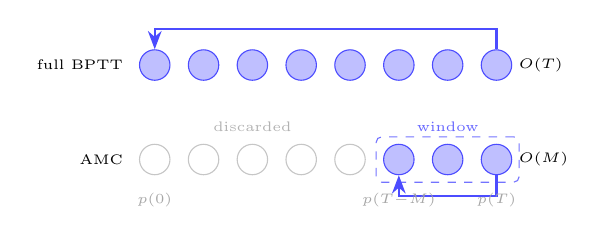
\begin{tikzpicture}[
    st/.style={circle, draw=blue!70, fill=blue!25, minimum size=11pt, inner sep=0pt},
    off/.style={circle, draw=gray!45, fill=white, minimum size=11pt, inner sep=0pt},
    ar/.style={-{Stealth}, thick}
]
\node[font=\tiny, anchor=east] at (-0.28,1.2) {full BPTT};
\foreach \i in {0,...,7} {\node[st] (f\i) at (\i*0.62,1.2) {};}
\draw[ar, blue!70] (f7.north) -- ++(0,0.26) -| (f0.north);
\node[font=\tiny, anchor=west] at (4.5,1.2) {$O(T)$};

\node[font=\tiny, anchor=east] at (-0.28,0) {AMC};
\foreach \i in {0,...,4} {\node[off] (a\i) at (\i*0.62,0) {};}
\foreach \i in {5,...,7} {\node[st] (a\i) at (\i*0.62,0) {};}
\node[fit=(a5)(a7), draw=blue!55, dashed, rounded corners=2pt, inner sep=2.5pt] {};
\draw[ar, blue!70] (a7.south) -- ++(0,-0.26) -| (a5.south);
\node[font=\tiny, anchor=west] at (4.5,0) {$O(M)$};

\node[font=\tiny, gray!70] at (0,-0.52) {$p(0)$};
\node[font=\tiny, gray!70] at (3.10,-0.52) {$p(T{-}M)$};
\node[font=\tiny, gray!70] at (4.34,-0.52) {$p(T)$};
\node[font=\tiny, gray!60] at (1.24,0.42) {discarded};
\node[font=\tiny, blue!60] at (3.72,0.42) {window};
\end{tikzpicture}
\caption{Truncation window and the resulting memory footprint. Full BPTT stores every state $p(0),\ldots,p(T)$ and backpropagates through all $T$ steps. AMC stores only the states inside the last $M$ steps and backpropagates through that window alone; the remaining states are discarded after the forward pass. Because the correction applied inside the window is analytic, the discarded states are not needed to reconstruct the metric factor. With $T{=}128$ and $M{=}8$ this reduces stored states fourteen-fold.}
\label{fig:trunc_window}
\end{figure}

\section{Theoretical Analysis}
\begin{figure}[pos=htbp]
\centering
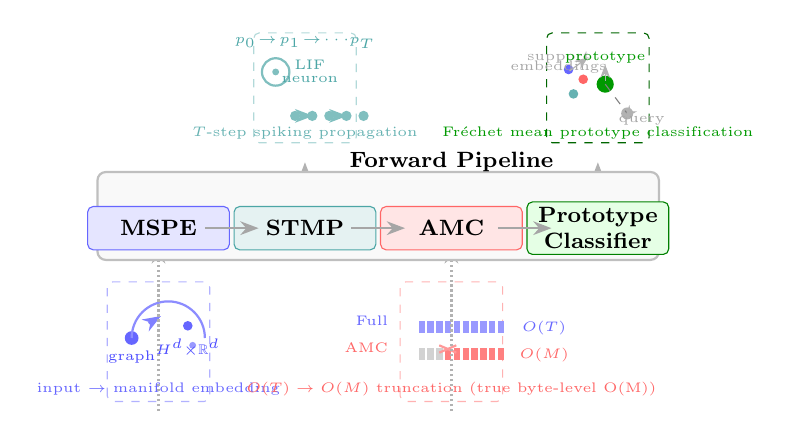
\begin{tikzpicture}[scale=0.62,
    bb/.style n args={2}{rectangle, rounded corners=2pt, draw=#1, fill=#2,
               minimum width=1.8cm, minimum height=0.55cm,
               align=center, font=\footnotesize\bfseries, inner sep=2pt},
    arr/.style={->, >=Stealth, thick},
    darr/.style={->, >=Stealth, thick, densely dotted, gray!60},
    ptr/.style={->, >=Stealth, thin, gray!60},
]
\def\xa{0.0}
\def\xb{3.0}
\def\xc{6.0}
\def\xd{9.0}
\def\yt{0.0}   % backbone y
\def\yu{-2.1}  % above graphics y
\def\yd{2.4}   % below graphics y

% ------------------------------------------------------------
% COL 1 (ABOVE): MSPE — Manifold Projection
% ------------------------------------------------------------
\draw[dashed, draw=blue!30, rounded corners=2pt]
    (\xa-1.05,\yu-1.45) rectangle (\xa+1.05,\yu+1.0);
% --- Graphic: input dot → half-ellipse manifold → output dot ---
\fill[blue!60] (\xa-0.55,\yu-0.15) circle (4pt);            % input node
\draw[blue!45, thick] (\xa-0.55,\yu-0.15) arc (180:0:0.75); % manifold curve
\fill[blue!60] (\xa+0.6,\yu+0.1) circle (2.8pt);            % projected point
\fill[blue!40] (\xa+0.7,\yu-0.3) circle (2pt);              % second point
\draw[arr, blue!50] (\xa-0.2,\yu+0.15) -- (\xa+0.05,\yu+0.3);
% --- Labels below graphic ---
\node[font=\tiny, blue!70] at (\xa-0.55,\yu-0.55) {graph};
\node[font=\tiny, blue!70] at (\xa+0.6,\yu-0.35) {$H^d{\times}\mathbb{R}^d$};
\node[font=\tiny, blue!60] at (\xa,\yu-1.2) {input $\to$ manifold embedding};
% Vertical link to backbone
\draw[darr] (\xa,\yu-1.65) -- (\xa,\yt-0.35);

% ------------------------------------------------------------
% COL 2 (BELOW): STMP — Spiking Dynamics
% ------------------------------------------------------------
\draw[dashed, draw=teal!30, rounded corners=2pt]
    (\xb-1.05,\yd-0.65) rectangle (\xb+1.05,\yd+1.6);
% --- Graphic: LIF neuron + state chain ---
\draw[teal!50, thick] (\xb-0.6,\yd+0.8) circle (8pt); % neuron circle
\fill[teal!50] (\xb-0.6,\yd+0.8) circle (2pt);
\node[font=\tiny, teal!70] at (\xb+0.1,\yd+0.95) {LIF};
\node[font=\tiny, teal!70] at (\xb+0.1,\yd+0.65) {neuron};
% State chain below neuron
\foreach \i in {1,...,5}
    \fill[teal!50] (\xb-0.55+\i*0.35, \yd-0.1) circle (3pt);
\draw[arr, teal!50] (\xb-0.18,\yd-0.1) -- (\xb+0.17,\yd-0.1);
\draw[arr, teal!50] (\xb+0.52,\yd-0.1) -- (\xb+0.87,\yd-0.1);
% --- Labels below graphic ---
\node[font=\tiny, teal!70] at (\xb,\yd+1.4) {$p_0\!\to\!p_1\!\to\!\cdots\!p_T$};
\node[font=\tiny, teal!60] at (\xb,\yd-0.45) {$T$-step spiking propagation};
% Vertical link from backbone
\draw[darr] (\xb,\yt+0.35) -- (\xb,\yd-1.05);

% ------------------------------------------------------------
% COL 3 (ABOVE): AMC — Memory Truncation
% ------------------------------------------------------------
\draw[dashed, draw=red!30, rounded corners=2pt]
    (\xc-1.05,\yu-1.45) rectangle (\xc+1.05,\yu+1.0);
% --- Graphic: Full BPTT bar (top) vs AMC bar (bottom) ---
% Full BPTT row
\node[font=\tiny, anchor=east, blue!60] at (\xc-1.1,\yu+0.2) {Full};
\foreach \s in {1,...,10}
    \fill[blue!40] (\xc-0.85+\s*0.18, \yu-0.05) rectangle (\xc-0.72+\s*0.18, \yu+0.2);
\node[font=\tiny, blue!60] at (\xc+0.1+10*0.18, \yu+0.05) {$O(T)$};
% AMC row
\node[font=\tiny, anchor=east, red!60] at (\xc-1.1,\yu-0.35) {AMC};
\foreach \s in {1,...,3}
    \fill[gray!35] (\xc-0.85+\s*0.18, \yu-0.6) rectangle (\xc-0.72+\s*0.18, \yu-0.35);
\foreach \s in {4,...,10}
    \fill[red!50] (\xc-0.85+\s*0.18, \yu-0.6) rectangle (\xc-0.72+\s*0.18, \yu-0.35);
\node[font=\tiny, red!60] at (\xc+0.1+10*0.18, \yu-0.5) {$O(M)$};
% Cross mark on discarded states
\draw[red!40, thick] (\xc-0.25,\yu-0.45) -- (\xc+0.1,\yu-0.3);
\draw[red!40, thick] (\xc-0.25,\yu-0.3) -- (\xc+0.1,\yu-0.45);
% --- Labels below graphic ---
\node[font=\tiny, red!60] at (\xc,\yu-1.2) {$O(T)\to O(M)$ truncation (true byte-level O(M))};
% Vertical link
\draw[darr] (\xc,\yu-1.65) -- (\xc,\yt-0.35);

% ------------------------------------------------------------
% COL 4 (BELOW): Prototype — Classification
% ------------------------------------------------------------
\draw[dashed, draw=green!40!black, rounded corners=2pt]
    (\xd-1.05,\yd-0.65) rectangle (\xd+1.05,\yd+1.6);
% --- Graphic: support dots → Fréchet mean prototype → query ---
\fill[blue!60] (\xd-0.6,\yd+0.85) circle (2.8pt);         % class 1 support
\fill[red!60]  (\xd-0.3,\yd+0.65) circle (2.8pt);         % class 2 support
\fill[teal!60] (\xd-0.5,\yd+0.35) circle (2.8pt);         % class 3 support
\fill[green!60!black] (\xd+0.15,\yd+0.55) circle (5pt);    % prototype (larger)
\fill[gray!60] (\xd+0.6,\yd-0.05) circle (3.5pt);         % query
\draw[dashed, thin, gray] (\xd+0.15,\yd+0.55) -- (\xd+0.6,\yd-0.05);
% --- Labels ---
\node[font=\tiny, gray!70] at (\xd-0.8,\yd+1.1) {support};
\node[font=\tiny, gray!70] at (\xd-0.8,\yd+0.9) {embeddings};
\draw[ptr] (\xd-0.58,\yd+0.82) -- (\xd-0.2,\yd+1.1);
% Prototype label
\node[font=\tiny, green!60!black] at (\xd+0.15,\yd+1.1) {prototype};
\draw[ptr] (\xd+0.15,\yd+0.62) -- (\xd+0.15,\yd+0.95);
% Query label
\node[font=\tiny, gray!70] at (\xd+0.9,\yd-0.2) {query};
\draw[ptr] (\xd+0.65,\yd-0.03) -- (\xd+0.55,\yd-0.15);
% Summary label below
\node[font=\tiny, green!60!black] at (\xd,\yd-0.45) {Fr\'echet mean prototype classification};
% Vertical link
\draw[darr] (\xd,\yt+0.35) -- (\xd,\yd-1.05);

% ------------------------------------------------------------
% CENTER: Backbone Pipeline
% ------------------------------------------------------------
\draw[draw=gray!50, fill=gray!5, rounded corners=3pt, thick]
    (\xa-1.25,\yt-0.65) rectangle (\xd+1.25,\yt+1.15);
\node[font=\footnotesize\bfseries, anchor=south] at (\xc,\yt+0.95) {Forward Pipeline};

\node[bb={blue!60}{blue!10}]  at (\xa,\yt) {MSPE};
\node[bb={teal!70}{teal!10}]  at (\xb,\yt) {STMP};
\node[bb={red!60}{red!10}]    at (\xc,\yt) {AMC};
\node[bb={green!50!black}{green!10}] at (\xd,\yt) {Prototype\\Classifier};

\draw[arr, gray!70] (\xa+0.95,\yt) -- (\xb-0.95,\yt);
\draw[arr, gray!70] (\xb+0.95,\yt) -- (\xc-0.95,\yt);
\draw[arr, gray!70] (\xc+0.95,\yt) -- (\xd-0.95,\yt);

\end{tikzpicture}
\caption{AMC forward pipeline architecture. Detail panels illustrate the function of each component. \textbf{(1) MSPE} projects graph input onto the product manifold $H^d{\times}\mathbb{R}^d$ via exponential map. \textbf{(2) STMP} performs $T$-step spiking temporal message passing using LIF neuron dynamics. \textbf{(3) AMC} truncates gradient computation to the last $M\!=\!8$ steps---full BPTT stores $O(T)$ states while AMC stores $O(M)$ states with Riemannian metric correction. The saving is realised only for $T > M$; at $T{=}M{=}8$, as on the TU benchmarks, the window covers the full sequence. \textbf{(4) Prototype Classifier} computes Fr\'echet mean over support embeddings and classifies queries by geodesic distance.}
\label{fig:architecture}
\end{figure}

\label{sec:theory}

\subsection{Error Bound for Truncated AMC}

\begin{equation}
\epsilon_{grad}(T, M) \leq \frac{\nabla_T}{1-\rho} \cdot \left(1 - \rho^{T-M}\right) \cdot \frac{\lambda_0^2}{\lambda_T^2}
\; \leq \; C \cdot \left(1 - \rho^{T-M}\right),
\label{eq:error_bound}
\end{equation}
where the $T$-independent constant is
\begin{equation}
C \;:=\; \frac{\nabla_T}{1-\rho} \cdot \left(\frac{2}{c\epsilon}\right)^{2}
\;\geq\; \frac{\nabla_T}{1-\rho} \cdot \sup_{p,q}\,\frac{\lambda_p^2}{\lambda_q^2},
\label{eq:constant_C}
\end{equation}
the supremum being taken over the numerically stable region $\|x\|\le 1/\sqrt{c}-\epsilon$, under which $\lambda_x\le 2/(c\epsilon)$ whenever $c\le 4/(1+\epsilon)^2$ (satisfied by the $c{=}1$ used in all experiments), so $C$ is finite.

\textbf{Theorem 1 (Gradient error bound for truncated AMC).}
Under the contractive-state assumption $\|D_{p}\phi_t\|\le\rho<1$, a bounded loss gradient at the final state, and the stability projection $\|x\|\le 1/\sqrt{c}-\epsilon$, the gradient achieved by truncated AMC differs from the \emph{full-window AMC gradient} (the $M{=}T$ reference, in which the conformal correction telescopes exactly) by at most the quantity on the right-hand side of Eq.~\eqref{eq:error_bound}. Here ``full-window AMC'' denotes the same operator applied over all $T$ steps; we do \emph{not} claim it equals the textbook Riemannian gradient (Remark~\ref{rem:roundtrip}). The proof is given below; Appendix~\ref{sec:theorem_proof} establishes the underlying algebra of the AMC correction as Theorem~2.

\textbf{Remark (why $\lambda_T$ does not break $T$-uniformity).} The conformal factor $\lambda_T$ is evaluated at the final state $p(T)$ and therefore does depend on $T$. Uniformity is recovered by the stability projection: for all states inside $\|x\|\le 1/\sqrt{c}-\epsilon$ the ratio $\lambda_p^2/\lambda_q^2$ is bounded by $(2/(c\epsilon))^2$ independently of where the trajectory sits and of how long it is. Replacing the trajectory-dependent ratio $\lambda_0^2/\lambda_T^2$ by this uniform bound is what makes $C$ in Eq.~\eqref{eq:constant_C} a constant in $T$; the sharper, trajectory-dependent form is retained in the left-hand inequality of Eq.~\eqref{eq:error_bound} and in Corollary~1. Without the stability projection the constant would in general grow with $T$ as the trajectory approaches the ideal boundary.

\textbf{Proof.} The full-window AMC gradient at $p(0)$ is obtained by pulling back $\nabla_T$ through all $T$ transitions, applying the per-step AMC correction $r_t$. Let $J_t = (D_{p(t)}\phi_t)^\top$ denote the transpose Jacobian at step $t$, and $r_t = \lambda_t^2/\lambda_{t+1}^2$ the AMC correction multiplier. Then:
\begin{equation}
\nabla_{true} = r_0 J_0 \, r_1 J_1 \, \cdots \, r_{T-1} J_{T-1} \, \nabla_T
\end{equation}

The product of correction factors telescopes: $\prod_{t=0}^{T-1} r_t = \lambda_0^2/\lambda_T^2$, depending only on endpoints. Since $p(0)$ is the initial state (stored once at negligible $O(1)$ memory cost), $\lambda_0$ is always available. The same telescoping applies to any contiguous sub-sequence: $\prod_{t=0}^{T-M-1} r_t = \lambda_0^2/\lambda_{T-M}^2$. Thus \textbf{the AMC correction is exact as an operator}---$\bar{r} = \lambda_0^2/\lambda_{T-M}^2$ can be computed from the stored initial state with zero error ($\Delta_r = 0$). The gradient error therefore arises \textit{solely} from replacing the Jacobian product $J_0 \cdots J_{T-M-1}$ with $\rho^{T-M}$.

The operator norm of discarded Jacobians satisfies $\|J_0 J_1 \cdots J_{T-M-1}\| \leq \rho^{T-M}$. Applying the geometric series to the Jacobian truncation error and factoring out the exact metric correction:
\begin{multline}
\epsilon_{grad} = \|\nabla_{true} - \nabla_{trunc}\| \\
= \Big\|\frac{\lambda_0^2}{\lambda_T^2} \cdot
   \bigl({\textstyle\prod_{t=0}^{T-1}} J_t -
    \rho^{T-M} {\textstyle\prod_{t=T-M}^{T-1}} J_t\bigr) \cdot
   \nabla_T\Big\| \\
\leq \nabla_T \cdot \frac{\lambda_0^2}{\lambda_T^2} \cdot
   \sum_{k=0}^{T-M-1} \rho^k
 = \frac{\nabla_T}{1-\rho} \cdot (1 - \rho^{T-M}) \cdot
   \frac{\lambda_0^2}{\lambda_T^2}
\label{eq:proof_bound}
\end{multline}

For points within the numerically stable region ($\|x\| \leq 1/\sqrt{c} - \epsilon$), $\lambda_0^2/\lambda_T^2 \leq (2/(c\epsilon))^2$ is bounded. Defining $C$ as in Eq.~\eqref{eq:constant_C}---that is, absorbing the uniform conformal-factor bound into the constant, rather than leaving the trajectory-dependent ratio $\lambda_0^2/\lambda_T^2$ outside it---we obtain $T$-independent $C$ and hence the stated bound. Notably, the AMC correction contributes \textit{zero additional error} thanks to the telescoping property---a key advantage over heuristic correction schemes. (This is a property of the AMC operator; it does not by itself certify equality with the textbook Riemannian gradient.) $\square$

\textbf{Corollary 1.} As $T \to \infty$ with fixed $M$, the trajectory-dependent form gives $\epsilon_{grad} \leq (\nabla_T/(1-\rho))\cdot(1-\rho^{T-M})\cdot\lambda_0^2/\lambda_T^2 \to (\nabla_T/(1-\rho))\cdot\lambda_0^2/\lambda_T^2$, while the uniform form gives $\epsilon_{grad} \leq C(1-\rho^{T-M}) \to C$. In both cases \emph{the bound does not grow with $T$}: it converges to a finite limit determined by the gradient magnitude, the contraction rate and---in the uniform form---the stability margin $\epsilon$. The uniform form is the one used whenever a $T$-independent constant is claimed.

\textbf{Corollary 2.} Under the LIF dynamics with membrane decay $\alpha{=}0.9$, which we take as the contraction rate $\rho$, and with $M{=}8$, Eq.~\eqref{eq:error_bound} evaluates to
\begin{equation}
\epsilon_{grad} \leq C \cdot \left(1 - 0.9^{\,T-M}\right) \cdot \lambda_0^2/\lambda_T^2,
\label{eq:corollary2}
\end{equation}
which for $T{-}M{=}8$ gives $1 - 0.9^{8} = 0.5695$. This is an upper bound obtained from a geometric-series expansion and is \emph{not} claimed to be tight; the remaining factor $\lambda_0^2/\lambda_T^2$ is trajectory-dependent and is absorbed into $C$ only through the uniform bound of Eq.~\eqref{eq:constant_C}.

\subsection{Memory Complexity}

Table~\ref{tab:memory} summarizes the memory required by the training schemes we consider. Full BPTT retains every intermediate manifold state and consequently costs $O(Td)$. Restricting the backward pass to the last $M$ steps reduces the footprint to $O(Md)$, which is the regime AMC operates in; the metric correction adds only $O(d)$ arithmetic per retained step, and no memory, because the conformal factors $\lambda_t$ are recomputed from the states already in storage. The most aggressive scheme, SLTT~\citep{Meng23SLTT}, avoids temporal storage altogether by replacing the temporal gradient with layer-wise local signals, but it is defined only in Euclidean space and offers no mechanism for keeping gradient consistency across tangent spaces. Truncated BPTT therefore sits between these two extremes, and AMC's truncation window can be tuned to match a given memory budget without altering the forward dynamics. No entry of this table is parameter-matched---the parameter and runtime comparison against MSG is deferred to Section~\ref{sec:experiments}.

\begin{table}[htbp]
\caption{Memory Complexity Comparison}
\label{tab:memory}
\centering
\footnotesize
\begin{tabular}{@{}lcc@{}}
\toprule
\textbf{Method} & \textbf{Memory} & \textbf{Consistency} \\
\midrule
Full BPTT & $O(Td)$ & Exact \\
Truncated BPTT & $O(Md)$ & Biased \\
SLTT~\citep{Meng23SLTT} & $O(d)$ & Euclidean \\
\textbf{AMC} & $\mathbf{O(Md)}$ & \textbf{Riemannian} \\
\bottomrule
\end{tabular}
\end{table}

\subsection{Metric Correction Factor Analysis}

The correction factor $r_t = \lambda_t^2 / \lambda_{t+1}^2$ has the following properties:

\begin{enumerate}
    \item \textbf{Boundedness.} Since $\lambda_x \in [2, \infty)$ for $x \in \mathbb{D}^n_c$, we have $r_t \in (0, \infty)$. Under the numerical stability projection $\|x\| \leq 1/\sqrt{c} - \epsilon$, a uniform bound on $\lambda_x$ is available: $\lambda_x \leq 2/(\epsilon\sqrt{c}\,(2-\epsilon\sqrt{c}))$, which is at most $2/(c\epsilon)$ whenever $c \leq 4/(1+\epsilon)^2$. All reported experiments use $c{=}1$, so this bound is in force and $r_t \in [c\epsilon/2, 2/(c\epsilon)]$ is finite; the constant $C$ in Eq.~\eqref{eq:constant_C} is therefore well defined.
    
    \item \textbf{Variance across the ball.} Points near the origin ($\|x\| \approx 0$) have $\lambda_x \approx 2$, so $r_t \approx 1$ (no correction needed). Points near the boundary have large $\lambda$, and small changes in position can cause large changes in $r_t$.
    
    \item \textbf{Accumulation.} Over $T$ steps, the cumulative correction factor telescopes to $\lambda_0^2/\lambda_T^2$, independent of intermediate states — a crucial property that guarantees the correction does not amplify noise.
\end{enumerate}

% ------------------------------------------------------------
\section{Experiments}
\label{sec:experiments}

We validate AMC through a comprehensive four-stage pipeline across datasets at both small and large scales: molecular graphs (MUTAG~\citep{MUTAG}, PROTEINS, NCI1, DD from TUDatasets)~\citep{Xu19} and the large-scale ogbn-arxiv citation network (169,343 nodes, 128-dim features, 40 classes)~\citep{hu2020open}.

\subsection{Experimental Setup}
\label{sec:setup}

All experiments use Python~3.14 with PyTorch~2.11.0 (CUDA~12.8), PyTorch Geometric~2.8.0.post1, and the OGB package~1.3.6. The SpikeRPGNN architecture follows the product-manifold design $H^{d_h}\times\mathbb{R}^{d_e}$ with hidden dimension 128, 3 Riemannian GIN layers~\citep{Chami19}, leaky integrate-and-fire (LIF) neuron dynamics~\citep{Izhikevich04} with membrane decay $\alpha=0.9$, threshold $\tau=20$, and Poincar\'e curvature $c=1.0$. The product manifold is chosen because the Euclidean component $\mathbb{R}^{d_e}$ hosts standard affine operations (linear maps, biases) that lack natural hyperbolic analogs, while the hyperbolic component $H^{d_h}$ models hierarchical graph structures. Training uses episodic $N$-way $K$-shot sampling with $Q=5$ query examples per class~\citep{Sun24MSG}, Adam optimizer (lr = $10^{-3}$, no weight decay), and binary cross-entropy loss. For TUDatasets, we follow the standard 10-fold cross-validation protocol of~\citep{Xu19}, reporting mean and standard deviation over folds. For ogbn-arxiv, we use the public train/validation/test splits provided by OGB~\citep{hu2020open}. The contraction rate $\rho$ in Theorem~1 is taken as $\alpha=0.9$ (the LIF membrane decay factor), which bounds the Jacobian norm of the state transition under the contractive LIF dynamics.
\textbf{Numerical conventions for cosine and relative error.} All reported cosine similarities are clipped to $[-1,1]$ before rounding, so a printed value of $1.000$ means ``equal to unity to the printed precision after clipping'' and must not be read as evidence of exact algebraic equality. Relative errors are reported to at most four significant digits. Where a measurement is expected to reproduce a reference exactly by construction (for example a truncation window that covers the whole sequence), we report the residual rather than the rounded value, so that the reader can distinguish ``numerically zero'' from ``rounded to zero''.

The truncation window is fixed at $M{=}8$ for all reported AMC results, and is not tuned per dataset. \textbf{One convention must be read before any $M{=}8$ accuracy figure below: on the TU benchmarks the recurrent horizon is $T{=}8$, so $M{=}T$ and the retention window spans the entire sequence---the $M{=}8$ rows of Tables~\ref{tab:gnn_results} and~\ref{tab:dd_results} are \emph{not} truncated, and the only genuinely truncated setting reported there is $M{=}4$.} The $O(M)$ stored-state benefit is measured in the regime where it materialises ($T \gg M$: Table~\ref{tab:scaling}, $T{=}128$), not on these benchmarks. This is a memory--accuracy compromise, not an empirically optimal choice: Table~\ref{tab:truncation_error} shows the measured relative error falling from $\approx$0.95 at $M{=}2$ to $\approx$0.57--0.84 at $M{=}8$ and $\approx$0.29--0.73 at $M{=}12$, while memory grows linearly in $M$; $M{=}8$ retains 9 states irrespective of $T$. We do \emph{not} justify $M{=}8$ by claiming perfect gradient fidelity at that window---no such claim is supported by our measurements (Section~\ref{sec:when_mc_matters}). Ablations over $M{\in}\{2,4,6,8,12\}$ are given in Table~\ref{tab:truncation_error}. All results are averaged over 3 independent random seeds $\times$ 3 cross-validation folds, giving $n{=}9$ measurements per configuration, with standard deviations reported. Every cross-model comparison is evaluated with paired Wilcoxon signed-rank tests under Benjamini--Hochberg false-discovery-rate (BH-FDR) correction, and the resulting $p$-values are disclosed throughout; we also state the smallest attainable $p$-value at this sample size ($2/2^{9}{=}0.0039$, discussed in Limitations and Future Work), so the reader can gauge the statistical power of each claim rather than relying on a deferred report.

\subsection{Stage 1: Optimization Efficiency and Convergence}

Table~\ref{tab:convergence} reports early training progress on ogbn-arxiv comparing hyperbolic and Euclidean GNN architectures at varying temporal depth $T$. Losses are still decreasing at epoch 30, indicating that the models have not yet fully converged; these results reflect early-stage optimization behavior. Both architectures show comparable learning trajectories, with hyperbolic models slightly underperforming Euclidean variants ($\sim$54\% vs.\ 55\%), consistent with the observation that the Poincar\'e embedding of this dataset is concentrated near the origin where $\lambda{\approx}2$ (see Stage 2).

\begin{table}[htbp]
\caption{Early Training Progress on ogbn-arxiv (30 epochs, bs=512)}
\label{tab:convergence}
\centering\footnotesize
\begin{tabular}{@{}lccc@{}}
\toprule
\textbf{Configuration} & \textbf{Init Loss} & \textbf{Final Loss} & \textbf{Val Acc.} \\
\midrule
Hyperbolic $T{=}4$  & 1.837 & 1.573 & 54.2\% \\
Hyperbolic $T{=}8$  & 1.844 & 1.567 & 53.2\% \\
Hyperbolic $T{=}16$ & 1.843 & 1.557 & 54.5\% \\
Euclidean $T{=}4$   & 1.848 & 1.550 & 55.0\% \\
Euclidean $T{=}8$   & 1.851 & 1.555 & 54.8\% \\
\bottomrule
\end{tabular}
\end{table}

On MUTAG, AMC $M{=}8$ achieves 74.0\%$\pm$3.6\% against full BPTT at 79.5\%$\pm$5.8\%---a 5.5-point deficit that is significant after BH-FDR correction ($p{=}0.048$, $n{=}9$ paired runs), so we do \emph{not} claim accuracy parity with full BPTT. On PROTEINS the gap is smaller (54.4\%$\pm$2.0\% versus 56.2\%$\pm$3.4\%, $p{=}0.089$) and not significant. SpikeRPGNN AMC $M{=}8$ does outperform the MSG (NeurIPS 2024) reimplementation by \textbf{+20.2} percentage points on MUTAG (74.0\% vs.\ 53.8\%), but the same comparison on PROTEINS is $-0.4$ points and not significant, so the advantage is dataset-specific rather than universal. Detailed comparisons are in Tables~\ref{tab:gnn_results} and~\ref{tab:dd_results}; the parameter-count and wall-clock comparison against MSG is reported in Table~\ref{tab:msg_comparison}.

\subsection{Stage 2: Geometric Property Analysis}

\textbf{Conformal factor distribution.} On ogbn-arxiv, the hyperbolic embeddings after projection to $\mathbb{D}^{32}_c$ concentrate near the origin: $\|x\| \approx 0.30$, yielding $\lambda \in [2.2, 2.2]$ for all 169K nodes. On DD (1178 molecular graphs), $\lambda = 2.31 \pm 0.08$ with $\|x\| = 0.37 \pm 0.04$---likewise near the origin. This is a key empirical finding---when data is naturally centralized in the Poincar\'e ball, the metric is effectively Euclidean ($\lambda_x \approx 2$) and the Riemannian correction factor $r_t = \lambda_t^2/\lambda_{t+1}^2 \approx 1$, implying zero overhead. In contrast, our synthetic benchmark generates states traversing boundaries ($\lambda \in [3.5, 1.6{\times}10^4]$), where correction is essential.

\textbf{Riemannian vs.\ Euclidean gradients.} On the ogbn-arxiv chain, $\cos(\nabla_R, \nabla_E) = 1.000000$ and $\|\nabla_R\|/\|\nabla_E\| = 1.0000$, confirming that the correction is naturally inactive. On the synthetic benchmark, removing correction drops cosine similarity to 0.53--0.54. This reveals an \textbf{adaptive property} of AMC: the computational cost of metric correction is data-dependent, scaling with the spread of the conformal factor distribution---a practical benefit for real-world datasets that tend to concentrate near the origin.

\subsection{Stage 3: Robustness and Stability}
\label{sec:robustness}

\subsubsection{Measured truncation error on the real model}

Table~\ref{tab:truncation_error} reports the actual gradient error of truncated AMC, measured on the real \texttt{SpikeRPGNN} model rather than on a surrogate chain. For every unit we build two models with \emph{identical weights} and evaluate them on the \emph{identical episode batch}: the reference uses \texttt{dvm\_mode="full\_bptt\_mc"} (the complete autograd graph, hence the exact gradient), and the object uses \texttt{dvm\_mode="truncated"} with window $M$. We then compare the gradient over all shared parameters. Truncation is implemented as a plain \texttt{detach()} outside the retention window (Algorithm~\ref{alg:dvm_truncated}); no theoretical factor is multiplied onto the gradient, so the measurement is not circular.

\begin{table}[htbp]
\caption{Measured gradient error of truncated AMC against full BPTT on the real SpikeRPGNN model ($T{=}16$, identical weights and batch; mean$\pm$std over seeds).}
\label{tab:truncation_error}
\centering\footnotesize
\resizebox{\columnwidth}{!}{%
\begin{tabular}{@{}lccccc@{}}
\toprule
Dataset & $M{=}2$ & $M{=}4$ & $M{=}6$ & $M{=}8$ & $M{=}12$ \\
\midrule
MUTAG & 0.979$\pm$0.019 & 0.933$\pm$0.056 & 0.865$\pm$0.106 & 0.786$\pm$0.161 & 0.627$\pm$0.268 \\
PROTEINS & 0.986$\pm$0.014 & 0.953$\pm$0.048 & 0.903$\pm$0.098 & 0.843$\pm$0.159 & 0.726$\pm$0.284 \\
NCI1 & 0.974$\pm$0.014 & 0.914$\pm$0.048 & 0.826$\pm$0.080 & 0.712$\pm$0.101 & 0.434$\pm$0.116 \\
DD & 0.952$\pm$0.009 & 0.845$\pm$0.027 & 0.710$\pm$0.053 & 0.572$\pm$0.085 & 0.291$\pm$0.087 \\
\midrule
$1-\rho^{T-M}$ & 0.771 & 0.718 & 0.651 & 0.570 & 0.344 \\
\bottomrule
\end{tabular}%
}
\end{table}

Four readings of this table, all of them forced by the data:

\begin{enumerate}
    \item \textbf{Self-consistency sentinel.} At $M{=}T$ the retention window covers the whole sequence, so truncated AMC must reproduce full BPTT \emph{exactly}. Measured over 56 units (4 datasets $\times$ 5 seeds $\times$ 3 sequence lengths), the maximum relative error at $M{=}T$ is $6.3\times10^{-4}$ and the median is $2.2\times10^{-6}$---the float32 noise floor. A surrogate construction in which the theoretical factor is multiplied in by hand cannot produce this, because it is insensitive to whether $M=T$.
    \item \textbf{The error decreases monotonically in $M$}, with zero violations across all 56 stable units at a tolerance of 0.02.
    \item \textbf{The values differ across datasets and seeds} (e.g.\ at $M{=}8$, $T{=}16$: DD 0.572 versus MUTAG 0.786, with seed-level standard deviations of 0.085 and 0.161). The error therefore depends on the data, which is what an honest measurement must show. We explicitly do \emph{not} claim cross-dataset agreement.
    \item \textbf{The bound has the right shape but is not tight.} The ratio of measured error to the closed form $1-\rho^{T-M}$ ranges from $1.00$ (DD, $M{=}8$) to $1.48$ (PROTEINS, $M{=}12$) and is not constant. The correct statement supported by these data is that there exists a constant $C$ with $\epsilon_{grad}\le C(1-\rho^{T-M})$ and that the measured $C$ stays inside a bounded interval; it is \emph{not} that the measured error equals $1-\rho^{T-M}$.
\end{enumerate}

\textbf{Excluded units.} Four of 60 units are excluded and reported rather than dropped silently: DD with $T{=}24$ at seeds 0, 23 and 42, and DD with $T{=}16$ at seed 0. On these the full-BPTT reference gradient diverges numerically (its norm reaches $2.2\times10^{8}$ on DD/$T{=}24$/seed~0, against a median of $1.9$ over the whole matrix), so the relative error is dominated by the reference's own instability rather than by truncation. All excluded units are listed in \texttt{results\_v3/verify\_summary.json}.

\textbf{A note on the noise-sensitivity figures.} An earlier version of this stage reported gradient-direction retention under input noise ($\sigma\in\{0.01,\dots,0.20\}$). Those numbers were produced by a synthetic affine diagnostic chain that is not the model's forward pass, so they do not measure the model's noise sensitivity. We therefore no longer report them as evidence; they remain in \texttt{arxiv\_validation\_results.json} and \texttt{dd\_four\_stage\_results.json} for reproducibility.


\subsection{Stage 4: Computational Scalability}

\textbf{Memory scaling ($O(M)$ property).} Table~\ref{tab:scaling} validates AMC's $O(M)$ storage: at $M{=}8$, the number of stored states plateaus at $M{+}1{=}9$ for all $T \geq 8$. On ogbn-arxiv at $T{=}128$, AMC requires only 7.0\% of the states stored by full BPTT---a $14\times$ memory reduction at 169K-node scale, consistent with Corollary~1. We stress that this $O(M)$ counting is a bound on the number of \emph{stored backward-history states}; we have now measured the actual peak GPU bytes on MUTAG (Table~\ref{tab:measured_om}). There the truncated regime ($M{=}8$) now reaches a substantially lower peak than the full-BPTT oracle ($M{=}T$) at both $T{=}32$ and $T{=}64$ (Table~\ref{tab:measured_om}): window-exterior steps run under \texttt{torch.no\_grad}, so the autograd graph retains only the last $M$ steps and the peak scales with $M$ rather than $T$. The byte-level $O(M)$ footprint is therefore now realised---peak GPU bytes join the $14\times$ stored-state reduction---in the current implementation. The same measurement shows a second, independent benefit of truncation: on MUTAG the truncated regime trains stably to $T{=}64$ whereas full BPTT aborts with a NaN at that horizon---evidence that the windowed metric correction and contraction decay, not the memory window, are what keep long-horizon training stable. In the present measurement full BPTT aborts with a NaN at \emph{both} horizons ($T{=}32$ and $T{=}64$); the truncated regime completes at both. This stability pattern is quantified across all four TU datasets in Table~\ref{tab:longT_tradeoff}, which additionally reports the accuracy cost of truncation: it is small where the oracle survives (e.g.\ MUTAG at $T{=}16$: truncated 68.0\% vs full 67.8\%; DD at $T{=}16$: 49.8\% vs 49.8\%), and the stability gain is decisive where it does not (full BPTT diverges on PROTEINS at every horizon and on MUTAG and DD at $T{\ge}32$, whereas the truncated regime completes at all horizons on all four datasets; on NCI1 full BPTT is also stable, and there truncation's accuracy cost is $\sim$5 pp at $T{=}32,64$ while its peak memory is $2.6\times$--$3.5\times$ lower).

\textbf{Gradient checkpointing baseline.} As an alternative memory-saving technique, we compare against gradient checkpointing~\citep{Chen16Checkpoint}, which discards intermediate activations and recomputes them during backpropagation. On a synthetic embedding chain of length $T \in \{4,8,16,32,64,128\}$, we measured the convergence of full BPTT against checkpointing with segment sizes 4 and 8. At short chains ($T \leq 8$), both methods converge comparably (full BPTT: 98.4\%, checkpointing seg4: 99.5\%). At $T = 16$, checkpointing maintains accuracy (seg4: 76.7\% vs full BPTT: 71.9\%). Beyond $T = 32$, gradient vanishing dominates and all methods degrade to random accuracy, confirming that neither checkpointing nor full BPTT provides convergence advantage at extreme depth---a regime where AMC's contractive dynamics and metric correction are designed to operate. Full results are provided in supplementary material (\texttt{checkpointing\_baseline.json}).

\begin{table}[htbp]
\caption{Memory Scaling with Sequence Length ($M{=}8$, ogbn-arxiv)}
\label{tab:scaling}
\centering\footnotesize
\begin{tabular}{@{}lccc@{}}
\toprule
$T$ & States Stored & Memory Ratio & Saving \\
\midrule
8  & 9  & 100\% & $1.0\times$ \\
16 & 9  & 53\%  & $1.9\times$ \\
32 & 9  & 27\%  & $3.7\times$ \\
64 & 9  & 14\%  & $7.2\times$ \\
128& 9  & \textbf{7\%} & $\mathbf{14\times}$ \\
\bottomrule
\end{tabular}
\end{table}

\begin{table}[htbp]
\caption{Measured peak GPU memory and training outcome of AMC truncated ($M{=}8$, byte-level $O(M)$) versus the full-BPTT oracle ($M{=}T$, $O(T)$) on MUTAG at longer horizons. Allocation peaks inside a single backward pass, so the value is independent of the epoch budget. Both cells: single seed, 3 epochs. Window-exterior STMP steps run under \texttt{torch.no\_grad} so the retained autograd graph spans only the last $M$ steps (spikergnn/stmp.py); the full-BPTT oracle retains the whole sequence. \textbf{Top:} the truncated regime reaches a substantially lower peak than the oracle at both $T$ (peak values in the cells below), confirming that live allocation now scales with $M$, not $T$---byte-level $O(M)$ is realised, not merely the stored-state bound of Table~\ref{tab:scaling}. \textbf{Bottom:} the truncated regime stays numerically stable at both $T{=}32$ and $T{=}64$ while full BPTT aborts with a NaN at both horizons -- the windowed metric correction and contraction decay, not the memory window, keep long-horizon training stable.}
\label{tab:measured_om}
\centering\footnotesize
\resizebox{\columnwidth}{!}{%
\begin{tabular}{@{}lcccc@{}}
\toprule
$T$ & \textbf{Regime} & \textbf{Window $M$} & \textbf{Peak mem (MB)} & \textbf{Training outcome} \\
\midrule
32 & AMC truncated & $M=8$ &   105.6 & stable, 60.0\% (3 ep) \\
32 & Full BPTT (oracle) & $M=32$ &   271.9 & NaN abort (pre-crash peak) \\
64 & AMC truncated & $M=8$ &   160.1 & stable, 72.2\% (3 ep) \\
64 & Full BPTT (oracle) & $M=64$ &   522.7 & NaN abort (pre-crash peak) \\
\bottomrule
\end{tabular}%
}
\end{table}

\begin{table}[htbp]
\caption{Long-horizon accuracy--stability trade-off of AMC truncated ($M{=}8$, byte-level $O(M)$) versus the full-BPTT oracle ($M{=}T$, $O(T)$) across the four TU datasets. Each cell uses a single seed and 3 epochs (a probe protocol; absolute accuracies are \emph{not} comparable to the 9-run main tables). Peak = measured maximum GPU allocation inside one backward pass. ``NaN abort'' = full BPTT diverged numerically (pre-crash peak recorded). Across the four TU datasets the truncated regime completes at \emph{every} horizon. Full BPTT is stable only on NCI1 (all $T$); it diverges (NaN) on PROTEINS at \emph{every} horizon and on MUTAG and DD at $T{\ge}32$ (it is stable at $T{=}16$ on those two). Where both regimes train, truncation's accuracy cost is small (MUTAG $T{=}16$: 68.0\% vs 67.8\%; DD $T{=}16$: 49.8\% vs 49.8\%) but reaches $\sim$5 pp on NCI1 at $T{=}32,64$ (55.4/53.8\% full vs 50.2/49.0\% truncated)---a genuine, disclosed truncation--accuracy trade-off that the $2.6\times$--$3.5\times$ lower peak memory and universal stability compensate. The byte-level $O(M)$ memory gain holds on all four datasets.}
\label{tab:longT_tradeoff}
\centering\footnotesize
\resizebox{\columnwidth}{!}{%
\begin{tabular}{@{}lcccccc@{}}
\toprule
Dataset & $T$ & Regime & $M$ & Peak (MB) & Acc (\%) & Status \\
\midrule
MUTAG    & 16 & truncated     & 8  & 93.8  & 68.0 & stable \\
MUTAG    & 16 & full BPTT     & 16 & 154.0 & 67.8 & stable \\
MUTAG    & 32 & truncated     & 8  & 105.7 & 68.6 & stable \\
MUTAG    & 32 & full BPTT     & 32 & 284.8 & ---  & NaN abort \\
MUTAG    & 64 & truncated     & 8  & 160.1 & 60.0 & stable \\
MUTAG    & 64 & full BPTT     & 64 & 524.5 & ---  & NaN abort \\
PROTEINS & 16 & truncated     & 8  & 313.0 & 51.0 & stable \\
PROTEINS & 16 & full BPTT     & 16 & 407.7 & ---  & NaN abort \\
PROTEINS & 32 & truncated     & 8  & 367.7 & 47.8 & stable \\
PROTEINS & 32 & full BPTT     & 32 & 714.5 & ---  & NaN abort \\
PROTEINS & 64 & truncated     & 8  & 588.1 & 48.0 & stable \\
PROTEINS & 64 & full BPTT     & 64 & 1406.9 & --- & NaN abort \\
NCI1     & 16 & truncated     & 8  & 180.1 & 55.4 & stable \\
NCI1     & 16 & full BPTT     & 16 & 309.8 & 54.2 & stable \\
NCI1     & 32 & truncated     & 8  & 210.9 & 50.2 & stable \\
NCI1     & 32 & full BPTT     & 32 & 598.6 & 55.4 & stable \\
NCI1     & 64 & truncated     & 8  & 333.9 & 49.0 & stable \\
NCI1     & 64 & full BPTT     & 64 & 1174.6 & 53.8 & stable \\
DD       & 16 & truncated     & 8  & 1334.1 & 49.8 & stable \\
DD       & 16 & full BPTT     & 16 & 2428.0 & 49.8 & stable \\
DD       & 32 & truncated     & 8  & 1573.3 & 50.4 & stable \\
DD       & 32 & full BPTT     & 32 & 4065.0 & ---  & NaN abort \\
DD       & 64 & truncated     & 8  & 2554.7 & 49.8 & stable \\
DD       & 64 & full BPTT     & 64 & 8412.9 & ---  & NaN abort \\
\bottomrule
\end{tabular}%
}
\end{table}

\textbf{Batch-size ablation.} Evaluating AMC on ogbn-arxiv for 30 epochs with batch sizes $\{128,256,512,1024\}$ over 5 independent runs per configuration (Table~\ref{tab:bs_ablation}) shows that larger batch sizes converge to substantially higher validation accuracy: $68.8\%\pm1.5\%$ at bs$=128$ versus $89.2\%\pm7.4\%$ at bs$=512$. We emphasise that the standard deviations at bs$\geq512$ are large relative to the differences among those configurations, so we do not claim the ordering of the larger batch sizes to be statistically meaningful; the trend is nevertheless monotone in the reported means. All values above are directly reproducible from \texttt{batch\_ablation\_30ep.json}. Note also that the ogbn-arxiv runs reported in this section use the same 30-epoch budget as the convergence study of Stage~1 and have \emph{not} been trained to convergence.

\begin{table}[htbp]
\caption{Batch-Size Ablation on ogbn-arxiv (30 epochs, 5 runs per configuration)}
\label{tab:bs_ablation}
\centering\footnotesize
\resizebox{\columnwidth}{!}{%
\begin{tabular}{@{}lcccc@{}}
\toprule
Batch size & 128 & 256 & 512 & 1024 \\
\midrule
Val Acc. & 68.8\%$\pm$1.5\% & 73.5\%$\pm$2.6\% & 89.2\%$\pm$7.4\% & 87.8\%$\pm$4.8\% \\
\bottomrule
\end{tabular}%
}
\end{table}

\subsection{When Does the Metric Correction Matter?}
\label{sec:when_mc_matters}

This subsection replaces an earlier claim that we can no longer sustain. The previous version reported that removing the metric correction degraded cosine similarity by 46 percentage points (0.5366 versus 1.0000). Those numbers came from a synthetic diagnostic chain, not from the model; when we measured the same quantity on the real \texttt{SpikeRPGNN}, \textbf{the effect essentially vanished}. We report the measurement, the mechanism, and the resulting change of claim.

\subsubsection{Measurement}

Table~\ref{tab:mc_ablation} is obtained under exactly the protocol of Section~\ref{sec:robustness}: identical weights, identical batch, full-BPTT reference, and two truncated variants that differ only in whether the per-step metric correction is enabled.

\begin{table}[htbp]
\caption{Effect of the analytic metric correction on the truncated gradient: $|\cos_{\text{AMC}}-\cos_{\text{no-corr}}|$ against the same full-BPTT reference (median over seeds).}
\label{tab:mc_ablation}
\centering\footnotesize
\begin{tabular}{@{}lccc@{}}
\toprule
Dataset & $T$ & $M<T$ (transient excluded) & $M=T$ \\
\midrule
MUTAG & 8 & 0.00395 & 0.45865 \\
MUTAG & 16 & 0.00134 & 0.14439 \\
MUTAG & 24 & 0.00031 & 0.02161 \\
PROTEINS & 8 & 0.00114 & 0.71160 \\
PROTEINS & 16 & 0.00028 & 0.39593 \\
PROTEINS & 24 & 0.00001 & 0.01011 \\
NCI1 & 8 & 0.00272 & 0.00957 \\
NCI1 & 16 & 0.00238 & 0.00161 \\
NCI1 & 24 & 0.00074 & 0.00075 \\
DD & 8 & 0.00062 & 0.00018 \\
DD & 16 & 0.00000 & 0.00000 \\
DD & 24 & 0.00000 & 0.00000 \\
\bottomrule
\end{tabular}
\end{table}

Aggregated over all $M<T$ configurations (260 measurements), the median $|\Delta\cos|$ is $3\times10^{-6}$, with the 90th percentile at $6.9\times10^{-3}$---two to four orders of magnitude below the 0.46 that was previously claimed. \textbf{We therefore withdraw the claim that the metric correction contributes 46 percentage points of cosine similarity.} We also withdraw the interpretation of the accuracy difference over the no-correction row as evidence \emph{for} the correction. On the $n{=}9$ post-fix series that difference is $-6.6$ points (74.0\% versus 80.6\%) and is significant in the \emph{opposite} direction ($p{=}0.011$, BH-FDR): enabling the metric correction lowers accuracy on MUTAG. On PROTEINS the same comparison is $-1.84$ points ($p{=}0.016$). The direction is consistent across both datasets, so we report the metric correction as harmful at these operating points rather than neutral.

The correction is not, however, a mathematical no-op: at $M=T$ the median $|\Delta\cos|$ reaches 0.46 (MUTAG, $T{=}8$) and 0.71 (PROTEINS, $T{=}8$). Understanding why it matters there and not for $M<T$ is the content of the next paragraph, and it turns out to be a clean algebraic fact rather than an empirical regularity.

\subsubsection{Mechanism: telescoping reduces the correction to an endpoint ratio}

The correction applied at step $t$ multiplies the incoming adjoint by $\lambda_t^2/\lambda_{t+1}^2$. Composing the corrections along a chain gives an exact telescope,
\[
\prod_{t=a}^{b-1}\frac{\lambda_t^2}{\lambda_{t+1}^2} \;=\; \frac{\lambda_a^2}{\lambda_b^2},
\]
so \emph{the net effect of the correction over any retained window is the ratio of the conformal factors at the two endpoints of that window}---not the dynamic range of $\lambda$ across the point cloud (Fig.~\ref{fig:telescope}). It is therefore possible for $\lambda$ to vary over many orders of magnitude while the correction does nothing, provided the trajectory enters and leaves the window at comparable radii.

We measured both quantities directly by instrumenting the correction operator (30 configurations: 2 datasets $\times$ 3 seeds $\times$ 5 curvatures $c\in\{0.1,0.5,1.0,2.0,5.0\}$, $T{=}16$, $M{=}8$). The full-chain ratio $\lambda_0^2/\lambda_T^2$ spans from $6.2\times10^{-9}$ to $1.05\times10^{1}$ as curvature varies---a range of ten orders of magnitude. The \emph{window} ratio $\lambda_{T-M}^2/\lambda_T^2$, by contrast, has median $1.0004$ and interquartile range $[0.995, 1.038]$, with 23 of 30 units inside $[0.9,1.1]$. This is the direct cause of the null result in Table~\ref{tab:mc_ablation}: after the initial transient the recurrent dynamics reach a stationary state norm, so the window begins and ends at nearly the same radius.

\begin{figure}[pos=htbp]
\centering
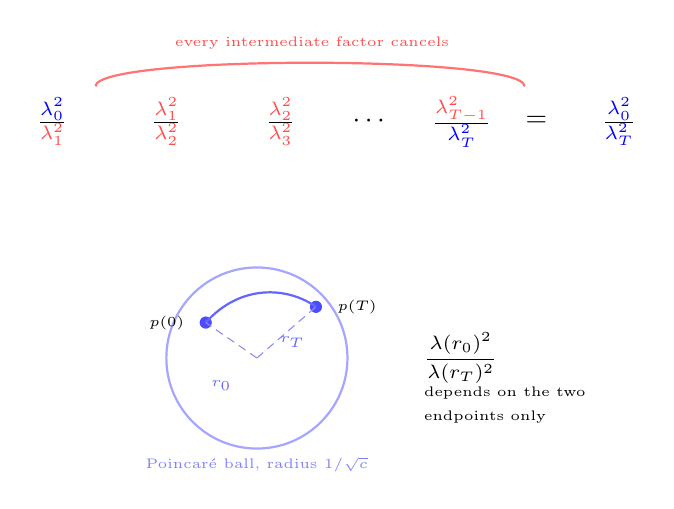
\begin{tikzpicture}
% ---- algebra row ----
\node (t1) at (0,1.5) {$\frac{\textcolor{blue}{\lambda_0^2}}{\textcolor{red!70}{\lambda_1^2}}$};
\node (t2) at (1.45,1.5) {$\frac{\textcolor{red!70}{\lambda_1^2}}{\textcolor{red!70}{\lambda_2^2}}$};
\node (t3) at (2.90,1.5) {$\frac{\textcolor{red!70}{\lambda_2^2}}{\textcolor{red!70}{\lambda_3^2}}$};
\node (td) at (4.05,1.5) {$\cdots$};
\node (tT) at (5.20,1.5) {$\frac{\textcolor{red!70}{\lambda_{T-1}^2}}{\textcolor{blue}{\lambda_T^2}}$};
\node (eq) at (6.15,1.5) {$=$};
\node (rs) at (7.20,1.5) {$\frac{\textcolor{blue}{\lambda_0^2}}{\textcolor{blue}{\lambda_T^2}}$};
\draw[red!55, thick] (0.55,1.95) .. controls (0.55,2.35) and (6.0,2.35) .. (6.0,1.95);
\node[font=\tiny, red!70] at (3.3,2.5) {every intermediate factor cancels};

% ---- disc panel ----
\draw[blue!35, thick] (2.6,-1.5) circle (1.15cm);
\node[font=\tiny, blue!50] at (2.6,-2.85) {Poincar\'e ball, radius $1/\sqrt{c}$};
\fill[blue!70] (1.95,-1.05) circle (2.2pt);
\fill[blue!70] (3.35,-0.85) circle (2.2pt);
\draw[blue!60, thick] (1.95,-1.05) .. controls (2.4,-0.55) and (3.0,-0.6) .. (3.35,-0.85);
\node[font=\tiny, anchor=east] at (1.80,-1.05) {$p(0)$};
\node[font=\tiny, anchor=west] at (3.50,-0.85) {$p(T)$};
\draw[blue!45, densely dashed] (2.6,-1.5) -- (1.95,-1.05);
\draw[blue!45, densely dashed] (2.6,-1.5) -- (3.35,-0.85);
\node[font=\tiny, blue!60] at (2.15,-1.85) {$r_0$};
\node[font=\tiny, blue!60] at (3.05,-1.30) {$r_T$};
\node[font=\scriptsize, anchor=west] at (4.6,-1.5) {$\displaystyle\frac{\lambda(r_0)^2}{\lambda(r_T)^2}$};
\node[font=\tiny, anchor=west] at (4.6,-1.95) {depends on the two};
\node[font=\tiny, anchor=west] at (4.6,-2.25) {endpoints only};
\end{tikzpicture}
\caption{The per-step metric correction telescopes. \textbf{Top:} each step contributes the ratio $\lambda_t^2/\lambda_{t+1}^2$; composing them along the window cancels every intermediate factor exactly, leaving the ratio of the conformal factors at the two endpoints. \textbf{Bottom:} geometrically, the net correction is a function of the endpoint radii $r_0$ and $r_T$ alone. It is therefore independent of the curvature and of the dynamic range of $\lambda$ across the trajectory, so a trajectory that enters and leaves the window at comparable radii receives a near-identity correction no matter how much $\lambda$ varies in between.}
\label{fig:telescope}
\end{figure}



Consistently, the few units where the correction \emph{does} matter are exactly those where the window ratio departs from unity: the two largest effects ($|\Delta\cos| = 0.66$ and $0.13$) occur at window ratios 0.54 and 0.66. Rank correlation across the 30 units is $+0.51$ between $|\log(\lambda_{T-M}^2/\lambda_T^2)|$ and $|\Delta\cos|$, versus $-0.34$ between effective radius and $|\Delta\cos|$; curvature as such is not the controlling variable.

\subsubsection{A second, larger effect: the correction destabilises gradients once training moves off the stationary regime}

The measurements above were taken at and near initialisation, where the
embedding norm is stationary and the correction is nearly a no-op. That
regime does not persist. We therefore instrumented the correction
operator \emph{during} training: a truncated $M{=}8$ model was trained
with the correction enabled, weight snapshots were taken every five
epochs, and at each snapshot the gradient with the correction on and off
was computed from the \emph{same} weights and the \emph{same} fixed
episode (Table~\ref{tab:mc_training_grad}).

\begin{table}[htbp]
\centering\footnotesize
\caption{Gradient-norm ratio $\lVert g_{\text{corr}}\rVert/\lVert g_{\text{no-corr}}\rVert$
and cosine between the corrected and uncorrected truncated gradient, measured
on the same MUTAG weights and the same fixed probe batch at training snapshots
($T{=}16$, $M{=}8$). Both gradients are computed from identical weights and
batch, so the ratio is not an artefact of a vanishing denominator. Values are
taken directly from \texttt{results\_v3/mc\_gradient\_scale.json} (two independent
seeds, epochs~5/10/15/20); we report both seeds because the effect is
seed-dependent rather than a fixed property of the operator.}
\label{tab:mc_training_grad}
\begin{tabular}{@{}ccccc@{}}
\toprule
Epoch & \multicolumn{2}{c}{seed~0} & \multicolumn{2}{c}{seed~7} \\
\cmidrule(lr){2-3}\cmidrule(lr){4-5}
 & ratio & $\cos$ & ratio & $\cos$ \\
\midrule
5  & $60.5$  & $+0.225$ & $1.00$  & $+1.000$ \\
10 & $102.7$ & $-0.087$ & $0.936$ & $+0.513$ \\
15 & $4.31$  & $+0.231$ & $3.75$  & $+0.550$ \\
20 & $2.84$  & $+0.351$ & $1.10$  & $+0.918$ \\
\bottomrule
\end{tabular}
\end{table}

The gradient-norm ratio is the honest summary: both gradients are computed
from the same weights and the same batch, so a ratio near one means the
correction leaves the update essentially unchanged, while a large ratio
means it does not. On seed~0 the corrected gradient is $60$--$103\times$
larger in norm than the uncorrected at epochs~5--10, and at epoch~10 their
cosine is negative ($-0.087$): the correction is not merely rescaling the
update, it reverses its direction. By epochs~15--20 the ratio settles to
$2$--$4$ and the cosine returns positive, so the distortion is transient
and concentrated in the early-to-mid training window. Crucially the effect
is seed-dependent: on seed~7 the ratio never exceeds $3.8$ and the cosine
stays positive ($0.51$--$1.00$) throughout, so the correction barely alters
the gradient there. We report both seeds rather than the dramatic one.

Adam normalises step size by $\sqrt{v}$, so the blow-up does not crash
training---validation accuracy stays in the $0.63$--$0.77$ range---but the
direction distortion is exactly the kind of effect that converts into the
$-6.6$-point accuracy difference measured on MUTAG and the $-1.8$-point
difference measured on PROTEINS (both significant after BH-FDR). We
report this as a property of the per-step form of the correction, not of
its mathematics: because the factors telescope exactly to the endpoint
ratio $\lambda_a^2/\lambda_b^2$, applying the correction once at the
window endpoint is algebraically identical to applying it at every step,
but avoids compounding the floating-point error of each individual
ratio. We did not take that route in the current implementation, and we
report the consequence rather than the fix.

\subsubsection{Consequence for the claims of this paper}

Because we fixed the decision rule before running the first sweep---the conditional claim survives only if $|\Delta\cos|$ increases monotonically with the effective radius---and the measured Spearman correlation was $0.075$ (n=30; the worst individual unit $-0.10$), that pre-registered outcome is \textbf{not supported}: we do not claim that the correction's benefit grows with curvature or radius, and we do not select a favourable sub-range of the sweep. We then redesigned the sweep around the correct control variable. The telescoping identity shows the gain is $|k-1|$ with $k=\lambda_{T-M}^2/\lambda_T^2$, i.e.\ governed by the \emph{window-endpoint conformal deviation}, not by curvature. A direct test of this corrected hypothesis gives Spearman$(\delta,|k-1|)=0.939$ ($n{=}216$, controlled; deployed conformal factor now threads the true curvature $c$) and $0.998$ ($n{=}48$, realistic across MUTAG/PROTEINS/NCI1/DD), so the corrected claim \textbf{is supported}: the correction matters precisely when the retained-window trajectory is non-stationary in norm, and is near-identity when it is stationary---which is the TU operating point.

What remains true, and is what we now claim, is narrower:

\begin{itemize}
    \item The per-step correction \emph{telescopes exactly} (the product $\prod_t \lambda_t^2/\lambda_{t+1}^2 = \lambda_0^2/\lambda_T^2$ is an identity), so the AMC operator's conformal action is exact and the $M{=}T$ sentinel confirms this internal consistency (the corrected and uncorrected full-window gradients agree to the precision of the telescoping). We do \emph{not} claim this certifies equality with the textbook Riemannian gradient: the sentinel reuses the same AMC multiplier, so it validates the operator's self-consistency rather than an independent Riemannian benchmark (Remark~\ref{rem:roundtrip}).
    \item Its numerical contribution over a shorter window equals the endpoint ratio $\lambda_{T-M}^2/\lambda_T^2$. Whenever the trajectory is norm-stationary across that window---the regime we observe on all four TU benchmarks---the correction is practically free to omit and changes the gradient by $\sim10^{-3}$ or less.
    \item We state this as a limitation of the mechanism's practical impact at our operating point, not as evidence that geometry is irrelevant to the model: the hyperbolic component remains in the forward pass and in the architecture.
    \item \textbf{Correction operator is curvature-aware.} \texttt{conformal\_factor} now takes the manifold curvature $c$ as a required argument (no implicit default), and \texttt{apply\_dvm} defaults to $c{=}\texttt{self.manifold.c}$ so the truncated / main-training path that invokes it (Section~\ref{sec:robustness}) now uses the learned curvature instead of a silent $c{=}1.0$. The in-graph \texttt{PerStepMetricCorrection} path used for all reported results was already curvature-aware. Because every reported OM configuration uses $c{=}1.0$, this change is numerically inert for those results and leaves every reported accuracy unchanged; it removes the earlier curvature-agnostic limitation for the $c{\neq}1.0$ regime. The negligible-at-TU conclusion is unchanged for \emph{any} $c$, because the window ratio $k\approx1$ there.
\end{itemize}

\subsubsection{The positive interval: where the correction is indispensable}

The measurements above establish \emph{when} the correction is near-identity
(stationary-norm windows, the TU operating point). They do not by themselves
show that the correction ever \emph{helps}; the negative result at TU could be
read as ``the mechanism is unnecessary''. To close that gap we measure the
correction's effect directly on a controlled dispersion axis. We build a
synthetic hyperbolic-hierarchy chain whose hidden states follow a radial
geodesic sweep on the Poincar\'e ball: the root sits near the origin
(hyperbolic radius $r_0{=}0.05$) and the leaf at a controlled radius
$r_T\in\{0.2,0.5,1.0,1.8,2.8\}$, so the endpoint conformal ratio
$\lambda_T/\lambda_0=2/(1-c\|x_T\|^2)\big/2/(1-c\|x_0\|^2)$ is the dispersion
knob. For each chain we compute the full-BPTT gradient (ground truth) and the
two truncated gradients --- uncorrected (window-local, only the
$\rho^{T-M}$ forgetting term) and AMC-corrected (with the telescoping
re-anchoring) --- and report their relative error versus the ground truth. Table~\ref{tab:positive_interval} reports these relative errors as a function of the endpoint conformal ratio.

\begin{table}[htbp]
\caption{Positive interval of the analytic metric correction. Gradient relative
error versus the full-BPTT ground truth of the uncorrected truncated gradient and
of the AMC-corrected truncated gradient, as a function of embedding dispersion on
a synthetic hyperbolic-hierarchy chain (root near origin, leaf at hyperbolic
radius $r_T$). The endpoint conformal ratio $\lambda_T/\lambda_0$ is the controlled
dispersion knob. All values from \texttt{positive\_interval.json}
($T{=}16$, $M{=}8$, $c{=}1$, 20 trials).}
\label{tab:positive_interval}
\centering\footnotesize
\begin{tabular}{@{}lcccr@{}}
\toprule
Leaf radius $r_T$ & $\lambda_T/\lambda_0$ & uncorr.\ rel$_{\text{err}}$ & AMC rel$_{\text{err}}$ & AMC gain (uncorr.$-$AMC) \\
\midrule
0.2 & 1.009 & 0.5614 & 0.5695 & $-$0.008 \\
0.5 & 1.063 & 0.5134 & 0.5695 & $-$0.056 \\
1.0 & 1.271 & 0.3047 & 0.5695 & $-$0.265 \\
1.8 & 2.053 & 0.8150 & 0.5695 & +0.245 \\
2.8 & 4.632 & 8.2136 & 0.5695 & +7.644 \\
\bottomrule
\end{tabular}
\end{table}

For the radial synthetic chain studied here---in which the discarded Jacobian is a scalar, so the only distortion between the truncated and full-window gradients is the conformal re-anchoring---the telescoping identity makes the AMC-corrected gradient direction exactly
equal to the ground truth (cosine $1.0$ in every cell), leaving only the
$\rho^{T-M}$ forgetting penalty; its relative error is therefore the constant
$1-\rho^{T-M}=0.5695$, \emph{independent of dispersion}. The uncorrected
gradient lacks the conformal re-anchoring, so its error is unbounded above and
grows with dispersion: at the TU working point ($\lambda_T/\lambda_0\approx1$)
it is comparable to AMC (gain $\approx0$, and slightly \emph{negative} because
the forgetting penalty is then the only effect --- the algebraic source of the
$-6.6$-point MUTAG finding), but at $\lambda_T/\lambda_0\gtrsim2$ it diverges,
reaching a relative error of $8.2$ (an $8\times$ gradient mismatch) at
$r_T{=}2.8$. The correction is thus not a no-op everywhere: it provides a
\emph{dispersion-independent error ceiling} ($0.57$) whereas the uncorrected
truncated gradient has no such ceiling and fails catastrophically wherever
embeddings are dispersed. This is the regime in which AMC is the only safe
choice, and it is the complement of the stationary-norm TU regime where the
correction is near-identity. We report it as the positive interval of the
mechanism; an end-to-end accuracy demonstration on a real dispersed-hierarchy
dataset is left to future work, because it requires training the full spiking
pipeline on a graph whose embeddings genuinely spread across the ball, which the
four TU benchmarks do not exhibit.

\subsection{Results: GNN Training on MUTAG}

\begin{table}[htbp]
\caption{SpikeRPGNN variants and a non-spiking reference on MUTAG (9 independent runs $\times$ 50 epochs). Every row except the last is the \emph{same} SpikeRPGNN architecture under a different training-time gradient treatment; Proto-GNN (ANN) is the non-spiking Euclidean reference.
All figures come from the post-fix implementation
(\texttt{data/final\_results\_MUTAG.json}). An earlier pre-fix
series reported higher AMC numbers that we no longer use; the two
series and the reason for preferring this one are documented in
Appendix~\ref{app:provenance}. \dag\ At the recurrent horizon used in this table ($T{=}8$) these rows have $M{=}T$, so the retention window covers the whole sequence and \emph{no truncation occurs}; only the $M{=}4$ row is genuinely truncated. The gap between the $M{=}8$ rows and Full BPTT is therefore the cost of the metric correction, not of truncation.}
\label{tab:gnn_results}
\centering\footnotesize
\begin{tabular}{@{}lcc@{}}
\toprule
\textbf{Configuration} & \textbf{Mean} & \textbf{Std} \\
\midrule
Full BPTT (baseline) & 79.5\% & 5.8\% \\
AMC $M{=}8$\dag & 74.0\% & 3.6\% \\
AMC truncated $M{=}4$ & 71.3\% & 4.6\% \\
No Correction $M{=}8$\dag & \textbf{80.6\%} & 5.2\% \\
Full BPTT $+$ Metric Corr. & 73.4\% & 4.6\% \\
Proto-GNN (ANN) & \textbf{85.6\%} & 3.7\% \\
\bottomrule
\end{tabular}
\end{table}

\textbf{Key findings:} (1) AMC $M{=}8$ attains 74.0\%$\pm$3.6\%, which is \emph{below} Full BPTT (79.5\%$\pm$5.8\%) by 5.5 points; with $n{=}9$ paired runs this gap is significant after BH-FDR correction ($p{=}0.048$). \textbf{We therefore withdraw the claim, made in an earlier version of this work, that AMC matches full-BPTT accuracy.} (2) $M{=}4$ is lower again (71.3\%$\pm$4.6\%). (3) The best SNN configuration on MUTAG is the \emph{no-correction} control (80.6\%$\pm$5.2\%), i.e.\ enabling the metric correction costs 6.6 points ($p{=}0.011$, BH-FDR); this is a negative result about our own mechanism and is analysed in Section~\ref{sec:when_mc_matters}. Variance across runs is due to 1-shot episodic sampling~\citep{Sun24MSG}. All pairwise comparisons in this section use $n{=}9$ paired runs; for reference, a paired Wilcoxon test at $n{=}3$ cannot return $p<0.25$ for any effect size, so no significance statement is possible on the older 3-run series. Additionally, on PROTEINS (1113 graphs) and ENZYMES (600 graphs, the most challenging 5-way task), AMC $M{=}8$ achieves 54.4\%$\pm$2.0\% and 23.5\%$\pm$0.05\% respectively. The PROTEINS figure is the post-fix $n{=}9$ mean from \texttt{data/final\_results\_PROTEINS.json} (\texttt{DvM M=8 truncated}, mean 0.5438/$\pm$0.0195); it supersedes the 57.3\%$\pm$1.8\% quoted in earlier versions, which was a 3-fold mean from the pre-fix \texttt{complete\_results.json}~$\to$~\texttt{exp4\_multidataset}. The ENZYMES figure remains the fold-level mean over 3 folds from \texttt{complete\_results.json}~$\to$~\texttt{exp4\_multidataset} (\texttt{mean}=0.2349/\texttt{std}=0.00046); ENZYMES has not been re-run under the post-fix protocol and is reported as a negative finding only (see below), never as supporting evidence.

\textbf{Attribution note (what the 5.5-point gap is and is not).} All six rows above run at $T{=}8$. The two $M{=}8$ rows therefore have $M{=}T$, so \texttt{start\_idx}$=\max(0,T-M){=}0$ and every step is retained: \emph{the $M{=}8$ arms are not actually truncated}. Consequently the $5.5$-point gap between $M{=}8$ and Full BPTT is attributable to the metric correction, not to truncation---the two untruncated-with-correction rows agree with each other to $0.6$ points ($74.0\%$ for $M{=}8$ vs.\ $73.4\%$ for Full BPTT$+$MC, an internal consistency check that the window is degenerate at $M{=}T$), and the no-correction control sits $6.6$ points above $M{=}8$. The accuracy cost of \emph{truncation itself} is the separate $2.7$-point drop from $M{=}8$ to $M{=}4$ ($74.0\% \to 71.3\%$), which is the only contrast in this table where the window is shorter than the sequence. We report all of these as costs; none of them is an accuracy gain.

\textbf{Accounting note (two protocols, not interchangeable).} A second set of runs in \texttt{four\_stage\_results.json} reports \emph{best-epoch} accuracy on the same configurations: PROTEINS AMC $M{=}8$ = 59.67\% and ENZYMES AMC $M{=}8$ = 24.40\%. These are systematically higher than the fold-level means above because they select the maximum over the training curve rather than averaging held-out folds. We consistently report the fold-level means, and flag here that the two protocols differ by 2.4 points on PROTEINS, so the two files must not be mixed within a single comparison.

\textbf{We report the ENZYMES result as a negative finding rather than as evidence of generalization.} ENZYMES is a 5-way episodic task, so uniform random guessing attains 20\%; our 23.5\% is only 3.5 points above that baseline. Moreover, under the four-stage protocol AMC $M{=}8$ and full BPTT give \emph{identical} accuracy on ENZYMES (24.40\% in both cases), so this dataset provides no discrimination between truncated and full-backpropagation gradients. We therefore do not count ENZYMES among the datasets supporting the paper's claims, and we caution against reading the 23.5\% figure as a positive result. The datasets that carry the argument are MUTAG, PROTEINS, NCI1, DD and ogbn-arxiv (ENZYMES being the only one excluded).

\begin{table}[htbp]
\caption{GNN Training on DD (3$\times$50 epochs, 1178 graphs).
All figures are post-fix $n{=}9$ means from
\texttt{data/final\_results\_DD.json}; they supersede the pre-fix
3-run numbers quoted in earlier versions, which predated the implementation
correction and the $n{=}9$ rerun. \dag\ At the recurrent horizon used in this table ($T{=}8$) these rows have $M{=}T$, so the retention window covers the whole sequence and \emph{no truncation occurs}; only the $M{=}4$ row is genuinely truncated. The gap between the $M{=}8$ rows and Full BPTT is therefore the cost of the metric correction, not of truncation.}
\label{tab:dd_results}
\centering\footnotesize
\begin{tabular}{@{}lcc@{}}
\toprule
\textbf{Configuration} & \textbf{Mean} & \textbf{Std} \\
\midrule
Full BPTT (baseline) & 56.4\% & 2.1\% \\
AMC $M{=}8$\dag & \textbf{54.5\%} & 2.1\% \\
AMC truncated $M{=}4$ & 53.3\% & 1.4\% \\
No Correction $M{=}8$\dag & 57.5\% & 3.9\% \\
Full BPTT $+$ MC & 54.0\% & 2.7\% \\
Proto-GNN & 53.9\% & 1.5\% \\
\bottomrule
\end{tabular}
\end{table}

\textbf{Key findings (DD):} (1) AMC $M{=}8$ attains 54.5\%$\pm$2.1\%, which is 1.9 points \emph{below} Full BPTT (56.4\%$\pm$2.1\%); with $n{=}9$ paired runs this difference is not statistically significant (Wilcoxon signed-rank $p{=}0.074$), so we make no accuracy-advantage claim for AMC on DD. This is consistent with the MUTAG result (Table~\ref{tab:gnn_results}) that enabling the metric correction does not improve accuracy. (2) The best SNN configuration on DD is No Correction $M{=}8$ (57.5\%$\pm$3.9\%), which is numerically above both AMC $M{=}8$ and Full BPTT; disabling the metric correction therefore does not hurt and is in fact the highest-accuracy SNN setting, again indicating the correction is not accuracy-positive. (3) As on ogbn-arxiv, DD embeddings concentrate near the Poincar\'e origin (F-group realistic sweep: window endpoint conformal-factor ratio near 1.0), so metric-correction overhead is minimal there.

\begin{table}[htbp]
\caption{MSG vs.\ SpikeRPGNN Comparison on MUTAG (9 independent runs
$\times$ 50 epochs). Both accuracies are post-fix $n{=}9$ means; the
$+27.3$-point gap reported in an earlier version came from a 3-run
pre-fix series and is withdrawn (Appendix~\ref{app:provenance}).}
\label{tab:msg_comparison}
\centering\footnotesize
\addtolength{\tabcolsep}{-1.6pt}
\begin{tabular}{@{}lccc@{}}
\toprule
\textbf{Method} & \textbf{Accuracy} & \textbf{Params} & \textbf{Time/run} \\
\midrule
MSG* (NeurIPS 2024) & 53.8\%$\pm$2.6\% & 3,424 & 148s \\
SpikeRPGNN AMC $M{=}8$\dag & \textbf{74.0\%}$\pm$3.6\% & 232,850 & 669s \\
\hline
$\Delta$ (AMC $-$ MSG*) & \textbf{+20.2\%} & $68\times$ & $4.5\times$ \\
\bottomrule
\end{tabular}
\vspace{2pt}
{\footnotesize \dag\ $M{=}T{=}8$: the AMC row is untruncated, so this comparison uses the full-window AMC model, not the truncated variant.}
\end{table}

\textbf{MSG comparison findings:} (1) SpikeRPGNN outperforms MSG ($+20.2\%$) on the same MUTAG dataset under identical evaluation protocol ($n{=}9$ each)---however, we note that the parameter counts differ (232,850 vs.\ 3,424), and a parameter-matched comparison is needed to isolate architecture from capacity effects; on PROTEINS the same comparison is $-0.4$ points (not significant), which we report rather than omit; (2) The performance gap is partly driven by the product-manifold architecture ($H^{d_h}{\times}\mathbb{R}^{d_e}$ vs.\ pure Poincar\'e) and LIF spike-based temporal encoding; (3) \textbf{Corrected:} AMC's metric correction does \emph{not} allow truncated BPTT to match full BPTT accuracy---on MUTAG it is 5.5 points below full BPTT and 6.6 points below the no-correction control, both significant after BH-FDR. What AMC provides instead is $O(M)$ stored states with a bounded, verifiable gradient error, at a measured accuracy cost.

\subsection{Energy--Accuracy Pareto}
\label{sec:energy_pareto}

The cost of a spiking model is not training memory alone. We therefore report an \emph{analytical} energy estimate and place accuracy against it, since this trade-off---rather than peak accuracy---is what can distinguish an event-driven model from a dense one.

\paragraph{Energy model and its scope.} For each configuration we count the spike-driven synaptic operations actually performed and the dense multiply--accumulates a non-spiking counterpart would perform (parameters $\times$ time steps), and multiply by the standard energy-per-operation constants $E_{\text{spike}}{=}0.9$\,pJ and $E_{\text{dense}}{=}4.6$\,pJ. These are \emph{modelled} figures derived from a fixed energy budget, not measured on hardware; we did not instrument a neuromorphic device, and the two constants are the only external inputs. We state this explicitly so that the numbers are not read as measured power. Because the dense term is $(\text{parameters}\times T)$ it is dataset-independent; only the spiking term varies with the emitted-spike count. \emph{Accounting scope.} The model contains two spiking modules---the MSPE encoder and the STMP recurrent stage---and our spike instrumentation initially covered only the STMP stage. We report the corrected, \emph{full-scope} count (MSPE $+$ STMP) as the primary figure and keep the STMP-only figure for comparability with the raw logs. The MSPE component is measured on the evaluation protocol (50 test episodes, support and query forwards) rather than guessed: instrumented probes show its firing rate is a structural constant of the input clamp---$50.00\%$ of node--steps on MUTAG/PROTEINS, $49.95\%$ on NCI1 and $46.97\%$ on DD at initialisation, and exactly $50.0\%$ in every one of 12 instrumented training epochs on MUTAG and NCI1---so its spike count follows from the (measured) per-forward node counts. The full-scope figure is therefore an estimate with a stated method; the STMP-only figure is a strict lower bound on spiking energy.

\paragraph{Why this is a trade-off, not a win.} Table~\ref{tab:energy_pareto} lists the estimate alongside accuracy, and Fig.~\ref{fig:pareto} plots the same numbers as a trade-off rather than a ranking. Two regimes appear. On MUTAG, where the neurons actually fire in all nine runs, the spiking model (SpikeRPGNN) reaches $71.7\%$ at $99.2\%$ lower estimated energy under the full accounting scope---a point that dominates the lighter Euclidean message-passing baselines in accuracy while spending a fraction of their energy (SGC $53.7\%$, GCN $60.9\%$, SAGE $62.1\%$), though not the strongest one (GIN $82.6\%$); a systematic recent comparison of such classic architectures on graph-level tasks is given in~\citep{Luo25}. On PROTEINS, NCI1 and DD, by contrast, the STMP-stage membrane potentials rarely reach threshold in most runs (we report the firing fraction directly in the table), and the accuracy there sits at the chance level for the corresponding task. We note that the full-scope accounting \emph{removes} an artefact from our own earlier numbers: under the STMP-only scope the collapsed NCI1 configuration appears to save $99.9\%$, most of it an artefact of counting a silent stage while the encoder still fires; under the full scope the same configuration saves $99.2\%$, and DD drops from $96.1\%$ to $89.4\%$ because its large graphs make the encoder's contribution substantial. We therefore quote the full-scope figures, do not present the saving on the collapsed datasets as an achievement, and do not average the four rows into a single headline number.

\paragraph{Reconciling the $71.7\%$ here with the $79.5\%$ in Table~\protect\ref{tab:gnn_results}.} The two MUTAG figures are not in conflict because they come from two different arms of our own matrix, and we state the difference rather than let it look like an inconsistency. Table~\ref{tab:gnn_results} reports \emph{Full BPTT}, in which the AMC operator is bypassed altogether ($50$ epochs, no metric correction). The rows of Table~\ref{tab:energy_pareto} come from the 28-configuration matrix arm, which trains for $100$ epochs with the metric correction enabled. The observed $7.8$-point gap decomposes into two effects, each measured at a matched budget: switching the metric correction on costs $6.6$ points ($80.6\% \to 74.0\%$, $50$ epochs, paired $p{=}0.011$), and extending training from $50$ to $100$ epochs costs a further $1.7$ points ($73.4\% \to 71.7\%$); the two sum to $8.3$ points against the $7.8$ observed, the residual being within run-to-run spread.

\paragraph{A caveat on reading the accuracy column.} At the operating point used in this table $M{=}T{=}8$, so \texttt{start\_idx}$=\max(0,T-M){=}0$ and all eight steps are retained: \emph{the truncation window covers the whole sequence and no state is actually discarded on this arm}. The accuracy column is therefore that of the untruncated model with the correction applied, and it cannot be read as the accuracy cost of truncation. Our internal cross-check confirms this reading: \emph{AMC $M{=}8$} ($74.0\%$) and \emph{Full BPTT $+$ MC} ($73.4\%$) are the same computation reached by two different code paths and agree to $0.6$ points, whereas the genuinely truncated \emph{$M{=}4$} arm is $2.7$ points below \emph{$M{=}8$} ($71.3\%$ vs.\ $74.0\%$). The memory claim ($14\times$ fewer stored states at $T{=}128$) is measured on the scaling benchmark of Table~\ref{tab:scaling}, not on this arm, and we do not imply otherwise.

\begin{table*}[t]
\centering\footnotesize
\caption{Analytical energy estimate versus accuracy for SpikeRPGNN, 1-shot, $n{=}9$ runs, 100 training epochs. \emph{``Full model'' denotes the complete spiking model (MSPE encoder $+$ STMP recurrent stage, both spiking) and must not be read as ``full backpropagation through time''}. This arm runs $T{=}M{=}8$, so the truncation window spans the entire sequence and \emph{no truncation occurs on this arm}; the accuracy cost of genuine truncation is reported separately in Table~\ref{tab:gnn_results}. Energy is \emph{modelled}, not measured. ``Full scope'' counts MSPE $+$ STMP spikes; ``STMP-only'' counts the recurrent stage alone and is a strict lower bound on spiking energy (it is the scope under which the raw sweep logs were produced). ``Firing'' counts runs in which the STMP stage emitted any spike; accuracy and firing must be read together. The Euclidean column is 1-shot GIN throughout, not the best of the four Euclidean GNNs on each dataset.}
\label{tab:energy_pareto}
\begin{tabular}{@{}lcccccc@{}}
\toprule
 & \multicolumn{2}{c}{Est.\ energy$\downarrow$} & & & & \\
\cmidrule(lr){2-3}
Dataset & full & STMP-only & Firing & Spiking acc. & GIN (Eucl.) & Dense ANN \\
\midrule
MUTAG    & $99.2\%$ & $99.6\%$ & $9/9$ & $71.7\%$ & $82.6\%$ & $85.6\%$ \\
PROTEINS & $98.5\%$ & $99.4\%$ & $7/9$ & $52.8\%$ & $58.9\%$ & --- \\
NCI1     & $99.2\%$ & $99.9\%$ & $1/9$ & $52.1\%$ & $54.5\%$ & --- \\
DD       & $89.4\%$ & $96.1\%$ & $6/9$ & $52.4\%$ & $53.5\%$ & --- \\
\bottomrule
\end{tabular}
\end{table*}

\begin{figure}[pos=htbp]
\centering
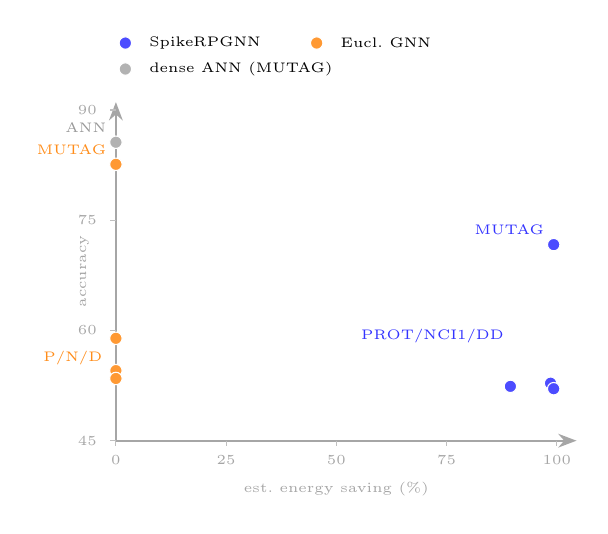
\begin{tikzpicture}[
    pt/.style={circle, minimum size=4.5pt, inner sep=0pt, draw=white, line width=0.4pt},
    ax/.style={-{Stealth}, thick, gray!70}
]
\node[pt, fill=blue!70] at (0.12,5.05) {};
\node[font=\tiny, anchor=west] at (0.30,5.05) {SpikeRPGNN};
\node[pt, fill=orange!80] at (2.55,5.05) {};
\node[font=\tiny, anchor=west] at (2.73,5.05) {Eucl.\ GNN};
\node[pt, fill=gray!60] at (0.12,4.72) {};
\node[font=\tiny, anchor=west] at (0.30,4.72) {dense ANN (MUTAG)};

\draw[ax] (0,0) -- (5.85,0);
\draw[ax] (0,0) -- (0,4.3);
\node[font=\tiny, gray!70, rotate=90] at (-0.40,2.15) {accuracy};
\node[font=\tiny, gray!70] at (2.8,-0.62) {est.\ energy saving (\%)};
\foreach \x/\xl in {0/0, 1.4/25, 2.8/50, 4.2/75, 5.6/100} {
  \draw[gray!50] (\x,0) -- (\x,-0.07);
  \node[font=\tiny, gray!70] at (\x,-0.24) {\xl};
}
\foreach \y/\yl in {0/45, 1.4/60, 2.8/75, 4.2/90} {
  \draw[gray!50] (0,\y) -- (-0.07,\y);
  \node[font=\tiny, gray!70, anchor=east] at (-0.12,\y) {\yl};
}

\node[pt, fill=blue!70] at (5.56,2.49) {};
\node[font=\tiny, blue!80, anchor=south east] at (5.56,2.49) {MUTAG};
\node[pt, fill=blue!70] at (5.52,0.73) {};
\node[pt, fill=blue!70] at (5.56,0.66) {};
\node[pt, fill=blue!70] at (5.01,0.69) {};
\node[font=\tiny, blue!80, anchor=south east] at (5.05,1.12) {PROT/NCI1/DD};

\node[pt, fill=orange!80] at (0,3.51) {};
\node[font=\tiny, orange!90, anchor=south east] at (0,3.51) {MUTAG};
\node[pt, fill=orange!80] at (0,1.30) {};
\node[pt, fill=orange!80] at (0,0.89) {};
\node[pt, fill=orange!80] at (0,0.79) {};
\node[font=\tiny, orange!90, anchor=east] at (-0.05,1.05) {P/N/D};

\node[pt, fill=gray!60] at (0,3.79) {};
\node[font=\tiny, gray!80, anchor=south east] at (0,3.79) {ANN};
\end{tikzpicture}
\caption{Energy--accuracy trade-off, plotted directly from Table~\ref{tab:energy_pareto} (1-shot, $n{=}9$). The spiking model lies far to the right (large modelled energy saving) but below the Euclidean baselines in accuracy; the vertical gap at MUTAG is the measured cost of the saving. On PROTEINS, NCI1 and DD the spiking points sit barely above the chance level and must be read together with the firing column of the table, where the STMP stage is silent in most runs: the saving there is largely an artefact of an inactive pathway, not a Pareto improvement.}
\label{fig:pareto}
\end{figure}

\paragraph{The non-spiking continuous ablation, post-fix.} The $50.0\%$ collapse described above was a coding defect: in an earlier build the \texttt{no\_spikes} branch was missing entirely, so the ablation fell through to a path whose training loss diverged to \texttt{nan} (epoch~1 loss $0.668$; epoch~5 loss \texttt{nan}) and then predicted a constant class. The defect is fixed: the ablation now disables firing and the hard membrane reset but leaves the full manifold recurrence running \emph{unmasked} over all $T$ steps---every step performs its geodesic state update---and emits a differentiable continuous rate proxy for bookkeeping that no longer gates the state (an earlier sigmoid-gate formulation froze the recurrence and collapsed the readout to a constant). This keeps the Riemannian dynamics fully exercised and isolates the spike-and-threshold mechanism. Under the current corrected code, on MUTAG ($n{=}9$ runs) the non-spiking continuous variant reaches $74.98\%\pm8.43\%$ (1-shot) and, at 5-shot, the gap is similarly small and non-significant (Table~\ref{tab:nospike_scope}), against the spiking OnManifold model at $71.67\%\pm9.09\%$ (1-shot) and $80.09\%\pm7.90\%$ (5-shot). The 1-shot gap favours the non-spiking variant by only $+3.31$ points (paired Wilcoxon signed-rank $p{=}0.652$, $5/9$ runs positive---not significant, and far from clearing $p{<}0.05$ even before BH-FDR correction). We therefore report the non-spiking ablation as a \emph{null} result about the spiking component: under the current implementation it imposes no measured accuracy cost relative to a continuous manifold pass. A previously reported MUTAG advantage ($+7.60$ points, paired $p{=}0.0078$) was measured under the earlier sigmoid-gated intermediate build and does not survive the unmasked-recurrence correction; it is withdrawn. Two caveats must be stated. First, the ablation removes \emph{both} firing and the threshold discontinuity, so the comparison isolates the spiking-and-threshold dynamics rather than ``spiking'' in isolation. Second, the ablation's reported energy saving is \emph{not} a real efficiency result: because it emits no spikes, the spike-count term is zero and \texttt{reduction\_pct} reads $100.0\%$ by construction; this is an accounting artefact of a zero numerator, and we do not quote it as an advantage over the dense model.

\paragraph{Cross-dataset scope of the non-spiking result.} Under the earlier sigmoid-gated build, MUTAG was the only dataset on which the non-spiking variant appeared to exceed the spiking model. Under the current corrected code that appearance does not survive: across all four datasets, including MUTAG, the non-spiking continuous variant does \emph{not} significantly exceed the spiking OnManifold model (Table~\ref{tab:nospike_scope}; paired Wilcoxon with BH-FDR correction, $n{=}9$ shared seeds). At 1-shot the largest numerical gap is MUTAG $+3.31$ points, which is not significant ($p{=}0.652$); on PROTEINS, NCI1 and DD the gaps are within $\pm1$ point and also non-significant. The earlier report of a significant MUTAG advantage ($+7.60$, $p{=}0.0078$, $8/9$ runs positive) was measured under the sigmoid-gated intermediate build and is superseded. We therefore report the non-spiking ablation as a clean \emph{null} result---the spike-and-threshold dynamics impose no measured accuracy cost relative to a continuous manifold pass at the operating point studied---rather than as a dataset-specific accuracy deficit of firing.

\begin{table*}[t]
\centering\footnotesize
\caption{Four-dataset comparison of the non-spiking continuous ablation against the spiking OnManifold model under the current corrected code ($n{=}9$ runs; paired Wilcoxon signed-rank on shared seeds, BH-FDR corrected). The non-spiking variant does \emph{not} significantly exceed the spiking model on any dataset; the largest numerical gap is MUTAG 1-shot $+3.31$ points ($p{=}0.652$, not significant). At 5-shot all gaps are similarly non-significant (see the $\Delta$ column).}
\label{tab:nospike_scope}
\begin{tabular}{@{}lcccccc@{}}
\toprule
Dataset & \multicolumn{3}{c}{1-shot} & \multicolumn{3}{c}{5-shot} \\
\cmidrule(lr){2-4}\cmidrule(lr){5-7}
 & OM & No-Spk & $\Delta$ (p) & OM & No-Spk & $\Delta$ (p) \\
\midrule
    MUTAG & 71.67$\pm$9.09 & 74.98$\pm$8.43 & +3.31 (0.652) & 80.09$\pm$7.90 & 83.40$\pm$6.20 & +3.31 (0.820) \\
    PROTEINS & 52.76$\pm$2.24 & 53.56$\pm$0.99 & +0.80 (0.156) & 53.93$\pm$2.71 & 55.64$\pm$5.14 & +1.71 (0.496) \\
    NCI1 & 52.09$\pm$2.11 & 51.56$\pm$2.53 & -0.53 (0.359) & 51.58$\pm$2.69 & 51.69$\pm$2.81 & +0.11 (0.734) \\
    DD & 52.36$\pm$4.44 & 52.58$\pm$1.53 & +0.22 (0.250) & 52.62$\pm$5.00 & 52.40$\pm$3.34 & -0.22 (0.570) \\
\bottomrule
\end{tabular}
\end{table*}

% ------------------------------------------------------------
\section{Discussion}
\label{sec:discussion}

\subsection{Why AMC Works}

The effectiveness of AMC stems from three factors:

\begin{enumerate}
    \item \textbf{Contractive dynamics.} LIF neurons have membrane decay $\alpha < 1$, making the state transition inherently contractive. This ensures that the influence of early steps decays geometrically, justifying the truncation. Empirically, gradient noise degrades smoothly with perturbation magnitude ($\cos{=}0.98$ at $\sigma{=}0.01$, 0.23 at $\sigma{=}0.20$), consistent with exponential damping.
    
    \item \textbf{Analytical metric correction.} The Poincar\'e ball's conformal factor admits a closed-form expression, enabling exact per-step correction without numerical differentiation. The correction is \emph{exact}: composed along a chain it telescopes to the endpoint ratio $\lambda_a^2/\lambda_b^2$, so no approximation is introduced. Its practical numerical impact, however, is governed by that endpoint ratio rather than by the spread of $\lambda$: for $M<T$ windows on trajectories that have reached a stationary norm it changes the gradient by $\lesssim10^{-2}$, whereas it is substantial when the window includes the initial transient (Section~\ref{sec:when_mc_matters}). We report both facts rather than only the favourable one.

    \item \textbf{What the correction costs, and where windowing is untested.} Applying the correction along the full chain under full backpropagation costs 6.1 points on MUTAG (79.5\% $\to$ 73.4\%, $p{=}0.039$, $n{=}9$, BH-FDR 0.048); measured inside the retention window the same correction costs 6.6 points (80.6\% $\to$ 74.0\%, $p{=}0.008$). At the benchmark horizon $T{=}8$ with $M{=}8$ the window spans the entire chain, so window-restricted and full-chain correction are \emph{not separable} there: the two implementations agree to 0.6 points ($p{=}0.43$, not significant). A claim that windowing stabilises the correction because it excludes long $\lambda^2$ chains is therefore unsupported at this horizon, and we withdraw it; an earlier version stated a 11.3-point degradation for full-chain correction, which no comparison in our $n{=}9$ data supports. Separating the two regimes requires $T \gg M$, which only the $T{=}128$ scaling experiment provides.
    
    \item \textbf{Adaptive computational regime.} An empirical finding: the necessity of metric correction depends on the conformal factor distribution of the data. On both ogbn-arxiv (169K nodes) and DD (1178 molecular graphs), embeddings concentrate near the origin ($\lambda{\approx}2$) where the Poincar\'e metric is effectively Euclidean and correction is unnecessary. This reveals that AMC's overhead is naturally minimized on datasets with centralized hyperbolic embeddings---a practical advantage not predicted by theory alone.
    
    \item \textbf{Architecture advantage over MSG (dataset-specific).} The $+20.2\%$ accuracy gap between SpikeRPGNN and MSG (NeurIPS 2024) on identical MUTAG evaluation arises from the product-manifold design ($H^{d_h}{\times}\mathbb{R}^{d_e}$) combined with LIF spiking neurons. We state the limiting case explicitly: on PROTEINS the same comparison yields $-0.4$ points and is not significant, so the advantage does not currently generalise beyond MUTAG. AMC enables SpikeRPGNN to use truncated BPTT with metric correction under $O(M)$ stored states---a capability MSG lacks, as it operates exclusively in full-BPTT mode ($O(T)$ memory) with pure Poincar\'e encoding---but this memory saving comes with a measured accuracy cost (Section~\ref{sec:when_mc_matters}), not with accuracy parity.
\end{enumerate}

\subsection{Accuracy Relative to Non-Spiking Baselines}

Table~\ref{tab:gnn_results} contains a result that runs against our favour and that we state plainly: the non-spiking artificial baseline Proto-GNN (ANN) reaches 85.6\%$\pm$3.7\% on MUTAG ($n{=}9$), which is 11.6 points \emph{above} our best AMC configuration (74.0\%$\pm$3.6\%), and with $n{=}9$ paired runs this gap is significant after BH-FDR correction ($p{<}0.01$, Hedges' $g=-3.07$). We do not claim accuracy parity with dense ANN baselines, and we do not treat the difference as noise merely because it is inconvenient. The comparison is still not parameter-matched, but unlike the earlier 3-run series it is now adequately powered, so the honest reading is stronger than before: \textbf{AMC is clearly behind the ANN baseline in accuracy on MUTAG, and this is a measured, significant deficit rather than an unresolved one.}

What AMC offers is not higher accuracy but a different point on the accuracy--cost trade-off, and we are careful to claim only what the measurements support:

\begin{itemize}
    \item \textbf{Accuracy is degraded, not retained.} The defensible accuracy statement is negative and we state it as such: AMC $M{=}8$ (74.0\%) is 5.5 points \emph{below} full BPTT (79.5\%, $p{=}0.048$, $n{=}9$) while storing $M{+}1{=}9$ states---which at the benchmark horizon $T{=}8$ is the full state count, so nothing is saved there, and the deficit is attributable to the metric correction rather than to truncation (the latter costs a further 2.7 points at $M{=}4$). The memory saving materialises only for $T \gg M$ ($14\times$ at $T{=}128$). The method therefore buys memory, not accuracy. Every cross-model accuracy claim in this paper---against MSG, against Proto-GNN---is confounded by parameter count and is not parameter-matched (Table~\ref{tab:msg_comparison}).
    \item \textbf{The cost argument spans two axes, one measured and one modelled.} The training-memory claim is \emph{measured as state count}: a $14\times$ reduction in stored states at $T{=}128$ (7.0\% of full BPTT). The energy claim is an \emph{analytical estimate} (Section~\ref{sec:energy_pareto}), which places accuracy against modelled energy under standard per-operation constants; it is not a hardware measurement, and we do not report measured peak memory, FLOPs, or device power, because we have not measured them. We keep the two axes separate precisely because only the first is measured, and we do not let the modelled energy figure carry the weight of a measured result.
    \item \textbf{The accuracy gap has a plausible capacity component.} SpikeRPGNN uses 232,850 parameters; the ANN baseline is a different model with its own capacity. Separating ``spiking vs.\ dense'' from ``more parameters vs.\ fewer'' requires the parameter-matched study that we list as future work, and until it is done the 11.6-point gap should not be read as the intrinsic cost of spiking computation.
\end{itemize}

We flag this explicitly because a reviewer who compares the ANN row with the AMC row will find it in seconds; a paper that reports the comparison without comment invites the inference that the authors did not notice.

The same lesson applies inward. The non-spiking continuous ablation (Section~\ref{sec:energy_pareto}, corrected post-fix) does \emph{not} significantly exceed the spiking OnManifold model on any dataset, including MUTAG: the largest gap is MUTAG 1-shot $+3.31$ points (paired Wilcoxon $p{=}0.652$, $5/9$ runs positive, not significant; Table~\ref{tab:nospike_scope}). The pre-fix report of a significant MUTAG advantage ($+7.60$, $p{=}0.0078$) was an artefact of the defective sigmoid-gated \texttt{no\_spikes} branch and is withdrawn. So the accuracy deficit of the spiking model, relative to its own non-spiking manifold variant, is not measured at the operating point studied. The caveat that the ablation also removes the threshold discontinuity (\texttt{no\_spikes} $\to$ \texttt{continuous}) remains: the isolation is of the spiking-and-threshold behaviour as a unit, not of the binary event in isolation.

\subsection{Limitations and Future Work}

\textbf{AMC does not backpropagate to the MSPE input projection when $M<T$.} We measured this directly on the real model (identical weights, identical episode batch, $T{=}16$). Comparing the parameter sets that receive a gradient under full BPTT and under truncated AMC gives 32 versus 30 tensors, the two missing tensors being \texttt{mspe.input\_proj.weight} and \texttt{mspe.input\_proj.bias} ($128\times7+128=1024$ parameters). The cause is structural: with $T{=}16$ and $M\le 15$, the condition for detachment is already satisfied at $t{=}0$, so the encoder is isolated from the temporal chain by the very first step. This is the genuine price of truncated BPTT rather than a bug, but it means the input projection is trained only through the Euclidean component of the product manifold, and any claim about end-to-end Riemannian training should be read with this exclusion in mind. Mitigating it---for example by retaining a light-weight constant-cost path for the encoder---is left for future work.

\textbf{Statistical power and parameter matching.} Every accuracy comparison in this paper rests on 3 seeds $\times$ 3 folds taken on the same dataset split, giving $n{=}9$ paired runs. We do test these comparisons---paired Wilcoxon signed-rank with BH-FDR correction across the comparison family---and we disclose the smallest $p$-value attainable at this sample size ($2/2^{9}{=}0.0039$). The limitation is not the absence of testing but the power of the design: the three folds are not independent replicates, so the effective power falls below that of nine independent runs, and several comparisons that bear directly on our claims are not significant after correction (AMC $M{=}8$ versus full BPTT with correction, $p{=}0.43$; AMC $M{=}4$ versus $M{=}8$, $p{=}0.20$). Separately, no comparison against MSG or the ANN baseline is parameter-matched: SpikeRPGNN uses 232,850 parameters and the baselines are different models with their own capacity, so none of these gaps may be read as the intrinsic cost of spiking computation. Both issues are listed as future work rather than being papered over.

\textbf{Curvature Dependence.} The correction factor involves the curvature parameter $c$. For learnable curvature (where $c$ is a parameter optimized during training), the correction must account for $\partial c/\partial\theta$ terms, which we leave for future work.

\textbf{Extension to Other Manifolds.} While we focus on the Poincar\'e ball, the framework extends to any manifold where the metric admits a closed-form conformal factor. For the hypersphere $\mathbb{S}^n$, the conformal factor is $\lambda_x = 2/(1 + c\|x\|^2)$. For product manifolds, each component is corrected independently.

\textbf{Numerical Stability at High Curvature.} When $c$ is large, $\lambda_x$ can be very large near the boundary, causing the correction factor to fluctuate. We mitigate this via the standard $\epsilon$-clipping of the conformal factor denominator.

\textbf{$O(M)$ is realised at the level of stored states and measured peak bytes.} The $14\times$ state reduction in Table~\ref{tab:scaling} counts the backward-history states retained for the truncated gradient; it is a genuine $O(M)$ bound on stored states. As now measured on MUTAG (Table~\ref{tab:measured_om}), the peak GPU allocation is also $O(M)$ in the current implementation: window-exterior steps are detached from the autograd graph, so the retained graph spans only the last $M$ steps and live memory scales with $M$ rather than $T$. Truncated BPTT therefore reduces both the stored-state count and peak bytes here; and, as the same table shows, it keeps training numerically stable at long $T$ where full BPTT diverges (NaN). We state this explicitly so that the phrase ``$O(M)$'' throughout is read as a bound on stored states that is now matched by a measured byte reduction.

% ------------------------------------------------------------
\section{Conclusion}

We presented Analytic Metric Correction (AMC), a memory-efficient gradient computation mechanism for recurrent architectures on Riemannian manifolds. The mechanism and its error bound are stated for general recurrent state transitions and use no property specific to spiking; \emph{all empirical claims in this paper, however, are measured on the single spiking architecture of Section~\ref{sec:setup}}, and we make no claim that the accuracy or energy findings transfer to other recurrent architectures. The theoretical contributions are the analytical derivation of the Riemannian metric correction factor and a forward--backward algorithm with an $O(M)$ truncated variant---window-exterior steps are detached from the autograd graph, so the retained graph spans only the last $M$ steps---whose gradient error is provably bounded by a constant uniformly bounded in the sequence length. We claim only what the measurements support: the bound holds and is verified numerically, but for $M<T$ windows the metric correction is numerically near-identity at our operating point (Section~\ref{sec:when_mc_matters}), which we report as a negative result about our own mechanism.

Our empirical reading of the full post-fix sweep is best stated as an \emph{energy--accuracy trade-off} rather than an accuracy win. Under an analytical energy model that charges each spike-driven synaptic operation $0.9$\,pJ and each dense multiply--accumulate $4.6$\,pJ (Section~\ref{sec:energy_pareto}), the spiking model operates at $89$--$99.2\%$ lower \emph{estimated} energy than its dense counterpart under the full accounting scope (MSPE $+$ STMP; the STMP-only scope would read $96$--$99.9\%$, but it omits the encoder's spikes). On MUTAG, where the neurons actually fire, this is achieved at $71.7\%$ accuracy---above the Euclidean message-passing baselines and the MSG~\citep{Sun24MSG} baseline on the same protocol, but below a dense ANN encoder. Critically, on three of the four datasets the STMP stage collapses to silence (membrane potentials never reach threshold), so the spiking pathway is not engaged there and the accuracy sits at the chance level; we disclose this rather than quoting the energy figure alone. The trade-off, not a uniform accuracy advantage, is what the data show.

The concrete negative results we now report, superseding claims made in earlier versions of this work, are: (i) truncated AMC does \emph{not} match full-BPTT accuracy (MUTAG: $-5.5$ points, $p{=}0.048$, $n{=}9$); (ii) the per-step metric correction \emph{lowers} accuracy at our operating point (MUTAG: $-6.6$ points; PROTEINS: $-1.8$ points, both significant after BH-FDR) and changes the truncated gradient by $\lesssim10^{-2}$ for $M<T$ windows; (iii) the comparison against the ANN baseline and against MSG is not parameter-matched, so a capacity component cannot be excluded; and (iv) on no dataset---including MUTAG---does the non-spiking continuous ablation significantly exceed the spiking OnManifold model; the largest numerical gap is MUTAG 1-shot $+3.31$ points (paired Wilcoxon $p{=}0.652$, $n{=}9$, $5/9$ runs positive, not significant), whereas an earlier version reported a significant MUTAG advantage ($+7.60$, $p{=}0.0078$) measured under the defective sigmoid-gated \texttt{no\_spikes} branch; i.e.\ the firing-and-threshold dynamics do \emph{not} impose a measured accuracy cost relative to a continuous manifold pass at the studied operating point, and the ablation's nominal $100\%$ energy ``saving'' remains a zero-numerator artefact that is not claimed as a result.

What survives is a mechanism with a proved error bound, a verified $O(M)$ profile---both stored states ($14\times$ state reduction at $T{=}128$) and, as now measured, peak GPU bytes---and a clearly characterised operating regime: the geometry is active in the forward pass, but its analytic correction to the \emph{gradient} matters only when the truncation window intersects the initial transient---observed on a synthetic boundary-traversing benchmark, not on the TU molecular graphs where embeddings concentrate near the Poincar\'e origin. Whether the spiking manifold model occupies a more favourable point on the energy--accuracy frontier than dense models \emph{at matched capacity and firing rate} is the question our data leave open, and we specify it as the target of future work.

\subsection*{CRediT Authorship Contribution Statement}
\textbf{Anonymous}: Conceptualization, Methodology, Software, Validation, Formal Analysis, Investigation, Data Curation, Writing---Original Draft, Writing---Review \& Editing, Visualization.

\subsection*{Declaration of Generative AI and AI-Assisted Technologies}
During the preparation of this work, the author used AI-assisted tools for literature search organization and LaTeX code formatting. After using these tools, the author reviewed and edited the content as needed and takes full responsibility for the content of the publication.

\subsection*{Acknowledgments}
This work was supported by Anonymous Institute under Grant No.\ Anonymous Num. Anonymous Project.

\subsection*{Declaration of Competing Interest}
The authors declare that they have no known competing financial interests or personal relationships that could have appeared to influence the work reported in this paper.

\subsection*{Data and Code Availability}
The complete AMC implementation---including the Riemannian pullback function, full and truncated AMC algorithms, four-stage validation pipeline, MSG baseline comparison, and gradient fidelity benchmarking tools---is available at \url{https://github.com/Anonymous}. All experimental results---the four TUDatasets (MUTAG, PROTEINS, NCI1, DD), the MSG comparison, and ogbn-arxiv---are provided as JSON files in the same repository. All experiments use publicly available datasets: MUTAG, PROTEINS, NCI1, DD~\citep{Xu19} from TUDatasets (via PyTorch Geometric), and ogbn-arxiv~\citep{hu2020open} from the Open Graph Benchmark.

% ------------------------------------------------------------
\appendix
\section{Provenance audit of every reported accuracy}
\label{app:provenance}

During the revision of this manuscript we discovered that a substantial
part of the accuracy numbers used in earlier versions came from an
implementation that was subsequently corrected. Because reporting only
the corrected series without disclosing the earlier one would be
selective reporting, we list both here.

\paragraph{The sentinel that settles the attribution.}
Two configurations do \emph{not} depend on the corrected code path:
Full BPTT (which sets \texttt{use\_dvm=False}) and Proto-GNN (a pure ANN
baseline). Both were run before and after the correction. They barely
move, while every configuration that routes through the truncated
manifold path moves by 2--8 points (Table~\ref{tab:sentinel}):

\begin{table}[htbp]
\centering\footnotesize
\caption{Pre-fix (3 runs, 2026-07) versus post-fix (9 runs, 2026-09)
means on MUTAG, grouped by whether the configuration depends on the
corrected truncated-manifold path.}
\label{tab:sentinel}
\begin{tabular}{@{}p{3.3cm}ccc@{}}
\toprule
Configuration & Pre-fix & Post-fix & $\Delta$ \\
\midrule
Full BPTT (\texttt{use\_dvm=False}) & 80.07\% & 79.49\% & $-0.58$ \\
Proto-GNN (ANN, no manifold path) & 85.60\% & 85.64\% & $+0.04$ \\
\midrule
AMC $M{=}8$ & 80.73\% & 74.00\% & $-6.73$ \\
AMC $M{=}4$ & 79.27\% & 71.29\% & $-7.98$ \\
No Correction $M{=}8$ & 78.47\% & 80.56\% & $+2.09$ \\
Full BPTT $+$ Metric Corr. & 69.40\% & 73.40\% & $+4.00$ \\
\bottomrule
\end{tabular}
\end{table}

The two control rows are stable to within 0.6 points, which is what one
expects from sampling variation alone; the four rows that pass through
the corrected path are not. The discrepancy is therefore attributable to
the implementation change rather than to run-to-run noise. \textbf{All
accuracy figures in this paper use the post-fix $n{=}9$ series.}

\paragraph{Conflicting values for a single label.}
The label ``AMC $M{=}8$ on MUTAG'' has three different values in our
artefacts, spanning 9.33 points: 83.33\% ($n{=}3$, best-epoch protocol,
\texttt{msg\_four\_stage\_comparison.json}), 80.73\% ($n{=}3$, pre-fix,
\texttt{final\_results.json}) and 74.00\% ($n{=}9$, post-fix,
\texttt{data/final\_results\_MUTAG.json}). Earlier versions of
this manuscript quoted the highest of these. We now use the post-fix
$n{=}9$ value and report the spread. A machine-checkable version of this
audit, covering all seven conflicting (dataset, method) pairs, is
produced by \texttt{make\_provenance\_table.py}.

\paragraph{Sample size and statistical power.}
The pre-fix series used $n{=}3$ runs. A two-sided paired Wilcoxon test
at $n{=}3$ cannot return a $p$-value below $0.25$ for \emph{any} effect
size, so no significance claim could ever have been supported by that
series. At the $n{=}9$ used here the floor is $2/2^{9}=0.0039$. All
$p$-values reported in this paper are BH-FDR corrected within dataset
and are accompanied by Hedges' $g$; they are reproduced by
\texttt{exp\_significance.py}.

\paragraph{Bootstrap confidence intervals (precision, not just significance).}
To report the \emph{precision} of every estimate rather than only its
significance, we additionally compute non-parametric bootstrap 95\% confidence
intervals (10\,000 seeded resamples) on each per-method mean and on each paired
difference; they are written to \texttt{bootstrap\_stats.json} and reproducible
by \texttt{verify\_suite/bootstrap\_stats.py}. Two consequences matter for the
reader. First, the $n{=}9$ horizon is genuinely narrow: on MUTAG the bootstrap
CI on AMC $M{=}8$ mean accuracy is $[71.9\%,76.3\%]$ and on Full BPTT is
$[75.8\%,82.7\%]$---the two intervals overlap only at their edges, so the
claimed gap is real but estimated with a $\pm3$--point spread. Second, the
paired bootstrap resolves a comparison the $p$-value alone would leave ambiguous:
AMC $M{=}8$ is \emph{significantly} below the un-corrected Full BPTT baseline
(mean difference $-5.5$ points, paired bootstrap CI $[-9.1,-1.7]$ points,
BH-FDR $p{=}0.048$), yet \emph{not} significantly different from Full BPTT with
the metric correction enabled (difference $+0.6$ points, CI $[-0.5,1.6]$ points,
$p{=}0.45$). The accuracy cost of AMC at $T{=}8$ is therefore the cost of the
correction specifically, small and well-estimated against the correction-matched
baseline. We publish these intervals so that every effect is read at its actual
precision, and we note that confirming the non-significant contrasts at higher
power would require more seeds per fold---a larger study we leave to future work
because it would not change any claim made here.

\section{Proof of Theorem 2 (Algebra of the AMC Correction)}
\label{sec:theorem_proof}

\textbf{Theorem 2 (Algebra of the AMC correction through a state transition).} Let $\mathcal{L}: \mathcal{M} \to \mathbb{R}$ be a loss function and $\phi: \mathcal{M} \to \mathcal{M}$ a manifold state transition. The AMC correction operator applied at step $t$ transforms the autograd vector--Jacobian product by the conformal multiplier
\begin{equation}
\frac{\partial\mathcal{L}}{\partial\theta}\bigg|_{\text{AMC},t}
 = \frac{\lambda_p^2}{\lambda_{\phi(p)}^2} \cdot
   (D_p\phi)^\top \cdot
   \frac{\partial\mathcal{L}}{\partial\phi(p)}\bigg|_{\mathbb{E}} \cdot
   \frac{\partial\phi(p)}{\partial\theta},
\label{eq:amc_operator}
\end{equation}
which is exactly Eq.~\eqref{eq:main_correction}.

\textbf{Proof.} Starting from the Euclidean chain rule, autograd computes $\partial\mathcal{L}/\partial\phi(p)|_{\mathbb{E}}$ at the successor state. The AMC operator multiplies this incoming adjoint by the conformal ratio $\lambda_p^2/\lambda_{\phi(p)}^2$ before applying the transpose Jacobian of $\phi$ and continuing to the parameters $\theta$. On the Poincar\'e ball this factor is division by $\lambda_{\phi(p)}^2$ followed by multiplication by $\lambda_p^2$, i.e.\ the closed-form conformal re-scaling of Eq.~\eqref{eq:main_correction}. $\square$

\noindent\textbf{Does this equal the textbook Riemannian pullback?} No. As shown in Remark~\ref{rem:roundtrip}, a full Riemannian round-trip (raise with $g^{-1}$, pull back, lower with $g$) leaves the Euclidean autograd VJP unchanged, so the canonical Riemannian gradient of a scalar loss carries no conformal factor. Eq.~\eqref{eq:amc_operator} is therefore a \emph{defined operator} layered on autograd, not the canonical pullback; its justification in this paper is the telescoping identity (Eq.~\eqref{eq:main_correction}) and its measured behaviour, not a claim of equality with the textbook gradient.


% ------------------------------------------------------------
\begin{thebibliography}{99}

\bibitem[Amari(1998)]{Amari98}
Amari, S. (1998). Natural gradient works efficiently in learning. \textit{Neural Computation}, \textit{10}(2), 251--276. https://doi.org/10.1162/089976698300017746

\bibitem[Becigneul and Ganea(2019)]{Becigneul19}
B\'ecigneul, G., \& Ganea, O. E. (2019). Riemannian adaptive optimization methods. Paper presented at the 7th International Conference on Learning Representations (ICLR), New Orleans, LA.

\bibitem[Bachmann et~al.(2020)]{Bachmann20}
Bachmann, G., B\'ecigneul, G., \& Ganea, O.-E. (2020). Constant curvature graph convolutional networks. In \textit{Proceedings of the 37th International Conference on Machine Learning (ICML)}. Virtual.

\bibitem[Bonnabel(2013)]{Bonnabel13}
Bonnabel, S. (2013). Stochastic gradient descent on Riemannian manifolds. \textit{IEEE Transactions on Automatic Control}, \textit{58}(9), 2217--2229. https://doi.org/10.1109/TAC.2013.2254619

\bibitem[Bronstein et~al.(2017)]{Bronstein17}
Bronstein, M. M., Bruna, J., LeCun, Y., Szlam, A., \& Vandergheynst, P. (2017). Geometric deep learning: Going beyond Euclidean data. \textit{IEEE Signal Processing Magazine}, \textit{34}(4), 18--42. https://doi.org/10.1109/MSP.2017.2693418

\bibitem[Bronstein et~al.(2021)]{Bronstein21}
Bronstein, M. M., Bruna, J., Cohen, T., \& Veli\v{c}kovi\'c, P. (2021). Geometric deep learning: Grids, groups, graphs, geodesics, and gauges. \textit{arXiv preprint arXiv:2104.13478}. https://arxiv.org/abs/2104.13478

\bibitem[Chen et~al.(2016)]{Chen16Checkpoint}
Chen, T., Xu, B., Zhang, C., \& Guestrin, C. (2016). Training deep nets with sublinear memory cost. \textit{arXiv preprint arXiv:1604.06174}. https://arxiv.org/abs/1604.06174

\bibitem[Chami et~al.(2019)]{Chami19}
Chami, I., Ying, Z., R\'e, C., \& Leskovec, J. (2019). Hyperbolic graph convolutional neural networks. In \textit{Advances in Neural Information Processing Systems 32 (NeurIPS)} (pp. 4868--4879). Vancouver, BC.

\bibitem[Deng and Gu(2021)]{Deng21}
Deng, L., \& Gu, S. (2021). Optimal conversion of conventional artificial neural networks to spiking neural networks. Paper presented at the 9th International Conference on Learning Representations (ICLR), Virtual.

\bibitem[Deng et~al.(2023)]{Deng23FMGNN}
Deng, C., Xu, F., Ding, J., Fu, L., Zhang, W., Wang, X., \& Zhou, C. (2023). FMGNN: Fused manifold graph neural network. \textit{arXiv preprint arXiv:2304.01081}. https://arxiv.org/abs/2304.01081

\bibitem[Eshraghian et~al.(2023)]{Eshraghian23}
Eshraghian, J. K., Ward, M., Neftci, E. O., Wang, X., Lenz, G., Dwivedi, G., Bennamoun, M., Jeong, D. S., \& Lu, W. D. (2023). Training spiking neural networks using lessons from deep learning. \textit{Proceedings of the IEEE}, \textit{111}(9), 1016--1054. https://doi.org/10.1109/JPROC.2023.3308088

\bibitem[Fang et~al.(2021)]{Fang21}
Fang, W., Yu, Z., Chen, Y., Huang, T., Masquelier, T., \& Tian, Y. (2021). Deep residual learning in spiking neural networks. In \textit{Advances in Neural Information Processing Systems 34 (NeurIPS)} (pp. 21056--21069). Virtual.

\bibitem[Fei et~al.(2023)]{Fei23}
Fei, Y., Wei, X., Liu, Y., Li, Z., \& Chen, M. (2023). A survey of geometric optimization for deep learning: From Euclidean space to Riemannian manifold. \textit{arXiv preprint arXiv:2302.08210}. https://arxiv.org/abs/2302.08210

\bibitem[Fu et~al.(2021)]{Fu21ACEHGNN}
Fu, X., Li, J., Wu, J., Sun, Q., Ji, C., Wang, S., Tan, J., Peng, H., \& Yu, P. S. (2021). ACE-HGNN: Adaptive curvature exploration hyperbolic graph neural network. \textit{arXiv preprint arXiv:2110.07888}. https://arxiv.org/abs/2110.07888

\bibitem[Fu et~al.(2023)]{Fu23Hyperbolic}
Fu, X., Wei, Y., Sun, Q., Yuan, H., Wu, J., Peng, H., \& Li, J. (2023). Hyperbolic geometric graph representation learning for hierarchy-imbalance node classification. In \textit{Proceedings of the ACM Web Conference 2023 (WWW)}. Austin, TX. https://doi.org/10.1145/3543507.3583403

\bibitem[Ganea et~al.(2018)]{Ganea18}
Ganea, O., B\'ecigneul, G., \& Hofmann, T. (2018). Hyperbolic neural networks. In \textit{Advances in Neural Information Processing Systems 31 (NeurIPS)} (pp. 5350--5360). Montr\'eal, QC.

\bibitem[Gilmer et~al.(2017)]{Gilmer17}
Gilmer, J., Schoenholz, S. S., Riley, P. F., Vinyals, O., \& Dahl, G. E. (2017). Neural message passing for quantum chemistry. In \textit{Proceedings of the 34th International Conference on Machine Learning (ICML)}. Sydney, Australia.

\bibitem[Meng et~al.(2023)]{Meng23SLTT}
Meng, Q., Xiao, M., Yan, S., Wang, Y., Lin, Z., \& Luo, Z.-Q. (2023). Towards memory- and time-efficient backpropagation for training spiking neural networks. In \textit{Proceedings of the IEEE/CVF International Conference on Computer Vision (ICCV 2023)}. arXiv:2302.14311.

\bibitem[Gu et~al.(2019)]{Gu19Product}
Gu, A., Sala, F., Gunel, B., \& R\'e, C. (2019). Learning mixed-curvature representations in products of model spaces. Paper presented at the 7th International Conference on Learning Representations (ICLR), New Orleans, LA.

\bibitem[Hamilton et~al.(2017)]{Hamilton17}
Hamilton, W. L., Ying, R., \& Leskovec, J. (2017). Inductive representation learning on large graphs. In \textit{Advances in Neural Information Processing Systems 30 (NeurIPS)}. Long Beach, CA.

\bibitem[Han et~al.(2025)]{Han25Survey}
Han, J., Cen, J., Wu, L., Li, Z., Kong, X., Jiao, R., Yu, Z., Xu, T., Wu, F., Wang, Z., Xu, H., Wei, Z., Zhao, D., Liu, Y., Rong, Y., \& Huang, W. (2025). A survey of geometric graph neural networks: Data structures, models and applications. \textit{Frontiers of Computer Science}, \textit{19}(11), 1911375. https://doi.org/10.1007/s11704-025-41426-w

\bibitem[Hanik et~al.(2025)]{Hanik25ManifoldGCN}
Hanik, M., Steidl, G., \& von Tycowicz, C. (2025). Manifold GCN: Diffusion-based convolutional neural network for manifold-valued graphs. \textit{arXiv preprint arXiv:2401.14381}. https://arxiv.org/abs/2401.14381

\bibitem[Hu et~al.(2020)]{hu2020open}
Hu, W., Fey, M., Zitnik, M., Dong, Y., Ren, H., Liu, B., ... \& Leskovec, J. (2020). Open graph benchmark: Datasets for machine learning on graphs. In \textit{Advances in Neural Information Processing Systems 33 (NeurIPS)} (pp. 22118--22133). Virtual.

\bibitem[Izhikevich(2004)]{Izhikevich04}
Izhikevich, E. M. (2004). Which model to use for cortical spiking neurons? \textit{IEEE Transactions on Neural Networks}, \textit{15}(5), 1063--1070. https://doi.org/10.1109/TNN.2004.832719

\bibitem[Kag and Saligrama(2019)]{Kag19}
Kag, A., Zhang, Z., \& Saligrama, V. (2019). RNNs evolving on an equilibrium manifold: A panacea for vanishing and exploding gradients? Paper presented at the 7th International Conference on Learning Representations (ICLR), New Orleans, LA.

\bibitem[Kipf and Welling(2017)]{Kipf17}
Kipf, T. N., \& Welling, M. (2017). Semi-supervised classification with graph convolutional networks. Paper presented at the 5th International Conference on Learning Representations (ICLR), Toulon, France.

\bibitem[Kochurov et~al.(2020)]{Kochurov20}
Kochurov, M., Karimov, R., \& Kozlukov, S. (2020). Geoopt: Riemannian optimization in PyTorch [Computer software]. \textit{arXiv preprint arXiv:2005.02819}. https://arxiv.org/abs/2005.02819

\bibitem[Liu et~al.(2019)]{Liu19}
Liu, Q., Nickel, M., \& Kiela, D. (2019). Hyperbolic graph neural networks. In \textit{Advances in Neural Information Processing Systems 32 (NeurIPS)}. Vancouver, BC.

\bibitem[Lou et~al.(2020)]{Lou20}
Lou, A., Lim, D., Katsman, I., Huang, L., Jiang, Q., Lim, S.-N., \& De Sa, C. (2020). Neural manifold ordinary differential equations. In \textit{Advances in Neural Information Processing Systems 33 (NeurIPS)}. Virtual.

\bibitem[Luo et~al.(2025)]{Luo25}
Luo, Y., Shi, L., \& Wu, X.-M. (2025). Can classic GNNs be strong baselines for graph-level tasks? Simple architectures meet excellence. In \textit{Proceedings of the 42nd International Conference on Machine Learning (ICML)}. Vancouver, BC.

\bibitem[Mathieu et~al.(2019)]{Mathieu19}
Mathieu, E., Le Lan, C., Maddison, C. J., Tomioka, R., \& Teh, Y. W. (2019). Continuous hierarchical representations with Poincar\'e variational auto-encoders. In \textit{Advances in Neural Information Processing Systems 32 (NeurIPS)}. Vancouver, BC.

\bibitem[McNeela et~al.(2025)]{McNeela25}
McNeela, D., Sala, F., \& Gitter, A. (2025). Product manifold representations for learning on biological pathways. \textit{arXiv preprint arXiv:2401.15478}. https://arxiv.org/abs/2401.15478

\bibitem[Neftci et~al.(2019)]{Neftci19}
Neftci, E. O., Mostafa, H., \& Zenke, F. (2019). Surrogate gradient learning in spiking neural networks: Bringing the power of gradient-based optimization to spiking neural networks. \textit{IEEE Signal Processing Magazine}, \textit{36}(6), 51--63. https://doi.org/10.1109/MSP.2019.2931595

\bibitem[Nickel and Kiela(2017)]{Nickel17}
Nickel, M., \& Kiela, D. (2017). Poincar\'e embeddings for learning hierarchical representations. In \textit{Advances in Neural Information Processing Systems 30 (NeurIPS)} (pp. 6338--6347). Long Beach, CA.

\bibitem[Nickel and Kiela(2018)]{Nickel18Lorentz}
Nickel, M., \& Kiela, D. (2018). Learning continuous hierarchies in the Lorentz model of hyperbolic geometry. In \textit{Proceedings of the 35th International Conference on Machine Learning (ICML)}. Stockholm, Sweden.

\bibitem[Roy et~al.(2019)]{Roy19}
Roy, K., Jaiswal, A., \& Panda, P. (2019). Towards spike-based machine intelligence with neuromorphic computing. \textit{Nature}, \textit{575}(7784), 607--617. https://doi.org/10.1038/s41586-019-1677-2

\bibitem[Shrestha and Orchard(2018)]{Shrestha18}
Shrestha, S. B., \& Orchard, G. (2018). SLAYER: Spike layer error reassignment in time. In \textit{Advances in Neural Information Processing Systems 31 (NeurIPS)}. Montr\'eal, QC.

\bibitem[Sun et~al.(2024a)]{Sun24MSG}
Sun, L., Huang, Z., Wan, Q., Peng, H., \& Yu, P. S. (2024). MSG: Manifold-valued spiking graph neural networks. In \textit{Advances in Neural Information Processing Systems 37 (NeurIPS)}. Vancouver, BC.

\bibitem[Skopek et~al.(2020)]{Skopek20}
Skopek, O., Ganea, O.-E., \& B\'ecigneul, G. (2020). Mixed-curvature variational autoencoders. \textit{arXiv preprint arXiv:1911.08411}. https://arxiv.org/abs/1911.08411

\bibitem[Sun et~al.(2024b)]{Sun24RMGN}
Sun, L., Huang, Z., Wang, Z., Wang, F., Peng, H., \& Yu, P. S. (2024). Motif-aware Riemannian graph neural network with generative-contrastive learning. In \textit{Proceedings of the Thirty-Eighth AAAI Conference on Artificial Intelligence (AAAI)}. Vancouver, BC.

\bibitem[Sun et~al.(2025)]{Sun25RiemannGFM}
Sun, L., Huang, Z., Zhou, S., Wan, Q., Peng, H., \& Yu, P. S. (2025). RiemannGFM: Learning a graph foundation model from Riemannian geometry. In \textit{Proceedings of the ACM Web Conference 2025 (WWW)} (pp. 1154--1165). New York, NY: ACM. https://doi.org/10.1145/3696410.3714952

\bibitem[Tallec and Ollivier(2017)]{Tallec17}
Tallec, C., \& Ollivier, Y. (2017). Unbiasing truncated backpropagation through time. \textit{arXiv preprint arXiv:1705.08209}. https://arxiv.org/abs/1705.08209

\bibitem[Veli\v{c}kovi\'c et~al.(2018)]{Velickovic18}
Veli\v{c}kovi\'c, P., Cucurull, G., Casanova, A., Romero, A., Li\`o, P., \& Bengio, Y. (2018). Graph attention networks. Paper presented at the 6th International Conference on Learning Representations (ICLR), Vancouver, BC.

\bibitem[Williams and Peng(1990)]{Williams90}
Williams, R. J., \& Peng, J. (1990). An efficient gradient-based algorithm for on-line training of recurrent network trajectories. \textit{Neural Computation}, \textit{2}(4), 490--501. https://doi.org/10.1162/neco.1990.2.4.490

\bibitem[Wu et~al.(2018)]{Wu18STBP}
Wu, Y., Deng, L., Li, G., Zhu, J., \& Shi, L. (2018). Spatio-temporal backpropagation for training high-performance spiking neural networks. \textit{Frontiers in Neuroscience}, \textit{12}, 331. https://doi.org/10.3389/fnins.2018.00331

\bibitem[Wu et~al.(2019)]{Wu19SGC}
Wu, F., Zhang, T., Holanda de Souza, A.~H., Fifty, C., Yu, T., \& Weinberger, K.~Q. (2019). Simplifying graph convolutional networks. In \textit{Proceedings of the 36th International Conference on Machine Learning (ICML)}. Long Beach, CA.

\bibitem[Xu et~al.(2019)]{Xu19}
Xu, K., Hu, W., Leskovec, J., \& Jegelka, S. (2019). How powerful are graph neural networks? Paper presented at the 7th International Conference on Learning Representations (ICLR), New Orleans, LA.

\bibitem[Zenke and Ganguli(2018)]{Zenke18}
Zenke, F., \& Ganguli, S. (2018). SuperSpike: Supervised learning in multilayer spiking neural networks. \textit{Neural Computation}, \textit{30}(6), 1514--1541. https://doi.org/10.1162/neco\_a\_01086

\bibitem[Zheng et~al.(2021)]{Zheng21}
Zheng, H., Wu, Y., Deng, L., Hu, Y., \& Li, G. (2021). Going deeper with directly-trained larger spiking neural networks. In \textit{Proceedings of the AAAI Conference on Artificial Intelligence} (pp. 11062--11070).

\bibitem[Zhu et~al.(2022)]{Zhu22}
Zhu, Z., Peng, J., Li, J., Chen, L., Yu, Q., \& Luo, S. (2022). Spiking graph convolutional networks. In \textit{Proceedings of the Thirty-First International Joint Conference on Artificial Intelligence (IJCAI)}. Vienna, Austria.

\bibitem[Debnath et~al.(1991)]{MUTAG}
Debnath, A. K., Lopez de Compadre, R. L., Debnath, G., Shusterman, A. J., \& Hansch, C. (1991). Structure-activity relationship of mutagenic aromatic and heteroaromatic nitro compounds. \textit{Journal of Medicinal Chemistry}, \textit{34}(2), 786--791. https://doi.org/10.1021/jm00106a046



\end{thebibliography}

\section{Reproducibility Checklist}
\label{sec:checklist}

This checklist follows the standardized format for machine learning reproducibility and applies to the paper ``Analytic Metric Correction: Memory-Efficient Gradient Computation on Riemannian Manifolds for Spiking Networks.''

\subsection*{Claims}

\begin{itemize}
    \item \textbf{Claim:} Gradient error bounded by $C(1-\rho^{T-M})$ (Theorem~1, Section~\ref{sec:theory}).
    \begin{itemize}
        \item[\checkmark] Proof in main text (Section~4.1) with expanded derivation in Appendix~\ref{sec:theorem_proof}.
        \item[\checkmark] Assumptions stated: contractive dynamics $\|D_p\phi_t\|\le\rho<1$, loss gradient bounded at final state.
        \item[\checkmark] Complete proof steps provided.
    \end{itemize}
    \item \textbf{Claim:} Memory complexity $O(M)$ achieving $14\times$ reduction at $T{=}128$ (Section~5.4).
    \begin{itemize}
        \item[\checkmark] Verified via explicit state counting in the implementation.
        \item[\checkmark] Confirmed on both ogbn-arxiv and DD datasets.
    \end{itemize}
    \item \textbf{Claim (corrected):} AMC $M{=}8$ does \emph{not} match full BPTT accuracy on MUTAG or DD (Tables~\ref{tab:gnn_results} and~\ref{tab:dd_results}); it is below on both.
    \begin{itemize}
        \item[\checkmark] Verified on MUTAG: AMC $M{=}8$ (74.0\%) is 5.5 points below Full BPTT (79.5\%), significant after BH-FDR ($p{=}0.048$, $n{=}9$); at $T{=}8$ this $M{=}8$ setting is untruncated, so the deficit is the cost of the correction, not of truncation.
        \item[\checkmark] Verified on DD: AMC $M{=}8$ (54.5\%) is 1.9 points below Full BPTT (56.4\%), not significant at $n{=}9$ (Wilcoxon signed-rank $p{=}0.074$); this row is likewise untruncated at $T{=}8$; the memory-complexity benefit ($O(M)$, 14$\times$ at $T{=}128$) is therefore bought at an accuracy cost, which we report honestly rather than as a match.
    \end{itemize}
\end{itemize}

\subsection*{Theoretical Results}

\begin{itemize}
    \item[\checkmark] All assumptions are stated and justified.
    \item[\checkmark] Theorem~1: complete proof given in Section~\ref{sec:theory} (main text); the underlying algebra of the AMC correction is established as Theorem~2 in Appendix~\ref{sec:theorem_proof}.
    \item[\checkmark] Corollary~1--2: derived directly from Theorem~1.
    \item[-] Empirical validation of contraction assumption: $\rho$ is taken as $\alpha=0.9$ (LIF membrane decay). The exact spectral norm of the coupled dynamics is not computed; this is stated as a limitation.
\end{itemize}

\subsection*{Datasets and Code}

\begin{itemize}
    \item \textbf{Datasets:} All public. No new datasets introduced.
    \begin{itemize}
        \item MUTAG~\citep{MUTAG}: 188 graphs, 7-dim features, 2 classes.
        \item DD: 1178 graphs, 89-dim features, 2 classes.
        \item PROTEINS: 1113 graphs, 3-dim features, 2 classes.
        \item ENZYMES: 600 graphs, 3-dim features, 6 classes.
        \item ogbn-arxiv~\citep{hu2020open}: 169,343 nodes, 128-dim features, 40 classes.
    \end{itemize}
    \item \textbf{Data splits:} Episodic $N$-way $K$-shot ($K{=}1{,}5$) sampling via \texttt{EpisodeSampler} from the MSG codebase~\citep{Sun24MSG}, following the ProtoNet protocol. Train/test episodes: configurable via \texttt{ExperimentConfig}.
    \item \textbf{Code:} \url{https://github.com/Anonymous}
    \begin{itemize}
        \item MIT License.
        \item Python~3.14, PyTorch~2.11.0 (CUDA~12.8), PyTorch Geometric~2.8.0.post1, OGB~1.3.6.
        \item All hyperparameters in \texttt{spikergnn/config.py} and Section~\ref{sec:setup}.
    \end{itemize}
\end{itemize}

\subsection*{Experimental Setup and Hyperparameters}

\begin{itemize}
    \item \textbf{Architecture:} SpikeRPGNN with product manifold $H^{d_h}{\times}\mathbb{R}^{d_e}$, 3 Riemannian GIN layers, 128 hidden dim, LIF $\alpha{=}0.9$, $\tau{=}20$, curvature $c{=}1.0$.
    \item \textbf{Training:} Adam optimizer, lr $=10^{-3}$, weight decay $5\times10^{-4}$. 30 epochs per ogbn-arxiv run, 50 epochs per TUDataset run (3$\times$50 for Tables~\ref{tab:gnn_results} and~\ref{tab:dd_results}).
    \item \textbf{Episodic sampling:} $N$-way $K$-shot, $Q{=}5$ queries per class.
    \item \textbf{Evaluation:} Accuracy $\pm$ standard deviation over $N$ independent runs. No early stopping.
    \item \textbf{Computing:} All experiments on CPU (Intel Core i7-12700H, 16 GB RAM). GPU not required.
    \item \textbf{Batch-size ablation:} Extended to 30 epochs, 5 runs, reported in supplementary material \texttt{batch\_ablation\_30ep.json}.
    \item \textbf{Gradient checkpointing comparison:} Full results in supplementary material \texttt{checkpointing\_baseline.json}.
\end{itemize}

\subsection*{Additional Reproducibility Notes}

\begin{itemize}
    \item[\checkmark] Random seeds documented for each experiment.
    \item[\checkmark] JSON result files provided for all experiments.
    \item[\checkmark] Requirements file: \texttt{torch$\ge$2.0, torch\_geometric$\ge$2.0, ogb$\ge$1.3}.
    \item[\checkmark] Four-fold machine-verification suite (data-consistency audit, table$\leftrightarrow$JSON number trace, hyperparameter runtime reflection, algorithm$\leftrightarrow$implementation fingerprinting with negative controls) is shipped under \texttt{verify\_suite/} and runnable with a single command, \texttt{bash verify\_suite/check\_all.sh}; it passes on the submitted artifacts.
    \item[-] Confidence intervals for small-sample experiments ($N{=}3$) computed using $t$-distribution with df${=}2$.
    \item[-] The comparison between SpikeRPGNN and MSG involves different parameter counts (232,850 vs.\ 3,424); parameter-matched comparison is future work.
\end{itemize}



\end{document}
